% 编译器：XeLaTeX
\documentclass[UTF8, 12pt]{ctexart}

% ===================== 页面与排版 =====================
\usepackage{geometry}
\geometry{
  a4paper,
  left=2.5cm, right=2.5cm,
  top=2.5cm,  bottom=2.5cm
}

% ===================== 数学 =====================
\usepackage{amsmath, amssymb, amsthm}
\newtheorem{theorem}{定理}[section]
\renewcommand{\proofname}{\textbf{证明}}
\newtheorem{lemma}{引理}[section]

% --- 自定义命令 ---
\newcommand{\norm}[1]{\left\|#1\right\|}
\newcommand{\inner}[2]{\left(#1, #2\right)}
\newcommand{\OmegaBar}{\overline{\Omega}}


% ===================== 图表 =====================
\usepackage{graphicx}
\usepackage{float}
\usepackage{booktabs}
\usepackage{caption}
\usepackage{multirow}
\captionsetup{font=small, labelfont=bf}

% ===================== 代码高亮 =====================
\usepackage{tcolorbox}
\tcbuselibrary{listings, breakable}
\usepackage{listings}
\usepackage{xcolor}

\lstset{
  language=Python,
  basicstyle=\ttfamily\small,
  keywordstyle=\color{blue!80!black}\bfseries,
  commentstyle=\color{green!50!black}\itshape,
  stringstyle=\color{red!60!black},
  numbers=left,
  numberstyle=\tiny\color{gray},
  numbersep=6pt,
  breaklines=true,
  frame=none,
  showstringspaces=false,
  tabsize=4,
}

% ===================== 超链接 =====================
\usepackage{hyperref}
\hypersetup{
  colorlinks=true,
  linkcolor=blue!70!black,
  citecolor=green!50!black,
  urlcolor=cyan!60!black,
}


% ===================== 杂项 =====================
\usepackage{enumitem}

% ===================== 标题信息 =====================
\title{\textbf{Robust-PINN for Optimal Control Problems}\\[6pt]
       \large Scaling 策略的有效性验证与状态约束扩展}
\author{兰景琪\\[2pt] \small Mathematics 2026}
\date{}

% ==================================================================
\begin{document}
\maketitle

\tableofcontents
\newpage

% ==================================================================
\section{从优化问题到一阶最优性系统：(1.1)--(1.2) 向 (1.3) 的转化}
\label{sec:derivation}

对于带有约束条件的函数优化问题，可以理解为求目标函数在约束条件下的极值问题，即条件极值。
从数学分析的角度来说，即使用 Lagrange 乘数法。
PDE 约束下的问题同样可以采用 Lagrange 乘数法，核心思想不变——将有约束的问题转化为无约束问题。
先构造 Lagrange 函数：
\[
  L(x,\lambda) = f(x) + \lambda \cdot g(x),
\]
其中 $g(x)$ 为等式约束，$f(x)$ 为目标函数，$\lambda \cdot g(x)$ 称为\textbf{惩罚项}。
再利用变分原理，求解无约束问题的极值。

\subsection{Lagrange 函数的构造}

本问题的目标函数为：
\begin{equation}
  J(\bar{y}, \bar{u})
  = \frac{1}{2}\|\bar{y} - y_d\|_{L^2(\Omega)}^2
  + \frac{\alpha}{2}\|\bar{u} - u_d\|_{L^2(\Omega)}^2,
  \label{eq:objective}
\end{equation}
约束状态为：
\begin{equation}
  g(\bar{y}) = -\Delta\bar{y} - f - \bar{u} = 0.
  \label{eq:constraint}
\end{equation}
在函数空间 $L^2(\Omega)$ 中，"函数相乘"被内积量化，惩罚项为：
\begin{equation}
  \langle p,\, g(y)\rangle_{L^2(\Omega)}
  = \int_\Omega p(x)\bigl(-\Delta y(x) - f(x) - \bar{u}(x)\bigr)\,\mathrm{d}x.
  \label{eq:penalty-term}
\end{equation}

另外，PDE 约束 $-\Delta y - f - \bar{u} = 0$ 的解 $y$ 需满足正则性（光滑性）。
在偏微分方程理论中，椭圆型 PDE 的 Dirichlet 问题的解属于 $H_0^1(\Omega)$ 空间，即
\[
  H_0^1(\Omega) = \bigl\{v \in L^2(\Omega) \,\big|\, \nabla v \in L^2(\Omega;\mathbb{R}^d),\;
  v\big|_{\partial\Omega} = 0\bigr\}.
\]
$p$ 作为伴随状态，同样要求在 $\partial\Omega$ 上 $p=0$，便于后续分部积分。

\subsection{对状态 $\bar{y}$ 的变分}

根据变分原理，最优解需满足 Lagrange 函数对各变量的 Fréchet 导数为零。

\paragraph{第一部分——目标函数对 $\bar{y}$ 的变分：}
\[
  \frac{\delta J}{\delta\bar{y}}
  = \frac{\partial}{\partial\bar{y}}\!\left(\frac{1}{2}\int_\Omega(\bar{y}-y_d)^2\,\mathrm{d}x\right)
  = \int_\Omega(\bar{y}-y_d)\,\delta\bar{y}\,\mathrm{d}x
  = \langle\bar{y}-y_d,\;\delta\bar{y}\rangle_{L^2}.
\]

\paragraph{第二部分——惩罚项对 $\bar{y}$ 的变分：}
利用 Green 第一公式：对任意 $u,v\in H_0^1(\Omega)$（边界上 $u=v=0$），有
\begin{equation}
  \int_\Omega \nabla u \cdot \nabla v\,\mathrm{d}x
  = -\int_\Omega v\,\Delta u\,\mathrm{d}x
  + \underbrace{\int_{\partial\Omega} v\,\nabla u \cdot \mathbf{n}\,\mathrm{d}S}_{\text{边界项}}.
  \label{eq:green}
\end{equation}
由于 $p$ 和 $\delta\bar{y}$ 在 $\partial\Omega$ 上均为零，边界项消失，因此
\[
  \int_\Omega p\,(-\Delta\delta\bar{y})\,\mathrm{d}x
  = \int_\Omega \delta\bar{y}\,(-\Delta p)\,\mathrm{d}x,
  \qquad\text{即}\quad
  \langle p,\,-\Delta\delta\bar{y}\rangle_{L^2}
  = \langle -\Delta p,\,\delta\bar{y}\rangle_{L^2}.
\]

\paragraph{合并：} 变分条件为
\[
  \delta\mathcal{L}
  = \langle\bar{y}-y_d,\;\delta\bar{y}\rangle_{L^2}
  + \langle -\Delta p,\;\delta\bar{y}\rangle_{L^2}
  = \langle\bar{y}-y_d - \Delta p,\;\delta\bar{y}\rangle_{L^2}
  = 0,
  \quad\forall\,\delta\bar{y}.
\]
由 $L^2$ 内积的非退化性，被积函数必须为零，从而得伴随方程：
\begin{equation}
  \boxed{-\Delta p = -(\ \bar{y} - y_d).}
  \label{eq:adjoint}
\end{equation}

\subsection{对控制 $\bar{u}$ 的变分}

目标函数对 $\bar{u}$ 的梯度为 $\langle\alpha(\bar{u}-u_d),\,\delta\bar{u}\rangle_{L^2}$，
惩罚项对 $\bar{u}$ 的梯度为 $-\langle p,\,\delta\bar{u}\rangle_{L^2}$。
合并得：
\[
  \langle\alpha(\bar{u}-u_d) - p,\;\delta\bar{u}\rangle_{L^2} = 0
  \quad\forall\,\delta\bar{u},
\]
从而
\begin{equation}
  p = \alpha(\bar{u} - u_d).
  \label{eq:control-eq}
\end{equation}

\begin{tcolorbox}[colback=blue!5!white, colframe=blue!60!black, title={注}]
如果问题的 Lagrange 函数定义为
$\mathcal{L}(y,u;p) = J(y,u) + \int_\Omega(\Delta y + f + u)\,p\,\mathrm{d}x$，
则一阶最优性系统为
\begin{equation}
  \begin{cases}
    -\Delta\bar{y} = f + \bar{u}  &\text{in } \Omega,\quad \bar{y}=0 \text{ on } \partial\Omega,\\
    -\Delta\bar{p} = \bar{y}-y_d  &\text{in } \Omega,\quad \bar{p}=0 \text{ on } \partial\Omega,\\
    \alpha(\bar{u}-u_d)+\bar{p}=0.
  \end{cases}
  \label{eq:kkt-alt}
\end{equation}
\end{tcolorbox}

\subsection{对伴随 $p$ 的变分}

Lagrange 函数中与 $p$ 相关的项仅为
$\langle p,\,-\Delta\bar{y}-f-\bar{u}\rangle_{L^2}$，
对 $p$ 求变分得：
\[
  \langle -\Delta\bar{y}-f-\bar{u},\;\delta p\rangle_{L^2} = 0
  \quad\forall\,\delta p,
\]
即得状态方程：
\begin{equation}
  \boxed{-\Delta\bar{y} = f + \bar{u} \quad\text{in } \Omega, \qquad \bar{y}=0 \quad\text{on } \partial\Omega.}
  \label{eq:state}
\end{equation}


% ==================================================================
\section{Scaling 处理对敏感性降低的有效性}
\label{sec:scaling-effectiveness}
\subsection{数值实验}
\label{sec:experiments}


% ============================================================
% 插入位置：scailing_report.tex 中 \section{Scaling 处理对敏感性降低的有效性}
%           \label{sec:scaling-effectiveness} 之后
% ============================================================

本节通过系统性的数值实验，验证 (1.5) 式 Scaling 变换对 PINN 求解椭圆最优控制问题时
降低参数敏感性的有效性。实验从两个维度展开：
\begin{itemize}
  \item \textbf{$\alpha$-敏感性}：固定损失函数权重，验证 Scaling 后误差对正则化参数
        $\alpha$ 的变化不敏感；
  \item \textbf{$\omega$-敏感性}：固定 $\alpha$ 于病态值 $10^{-4}$，验证 Scaling 后误差对
        损失函数全局权重 $\omega$ 的变化不敏感。
\end{itemize}


% ==================================================================
\subsection{实验设置}
\label{subsec:exp-setup}

\paragraph{精确解构造（MMS）。}
在 $\Omega = [0,1]^2$ 上取齐次 Dirichlet 边界条件，构造精确解
\[
  \bar{y}(x) = \sin(\pi x_1)\sin(\pi x_2), \qquad
  \bar{p}(x) = \alpha\sin(\pi x_1)\sin(\pi x_2).
\]
由最优性系统 (1.3) 反推源项及目标函数
\[
  f(x) = (2\pi^2 + 1)\,\bar{y}(x), \qquad
  y_d(x) = (1 - 2\pi^2\alpha)\,\bar{y}(x), \qquad
  u_d \equiv 0,
\]
以确保可精确定量验证。

\paragraph{网络架构。}
\begin{itemize}
  \item \textbf{Unified Network}（单网络双输出）：3 层隐藏层，每层 50 个神经元，
        SiLU 激活函数，输出维度为 2，分别表示 $y$ 和 $p$；
  \item \textbf{Dual Network}（双独立网络）：$y$ 和 $p$ 各由一个独立的同结构网络拟合，
        输出维度为 1。
\end{itemize}

\paragraph{边界条件处理。}
\begin{itemize}
  \item \textbf{硬边界（Hard BC）}：采用距离函数 Ansatz
        $\hat{y}(x) = D(x)\cdot N_\theta(x)$，
        其中 $D(x) = x_1(1-x_1)\,x_2(1-x_2)$，自动精确满足齐次 Dirichlet 边界条件；
  \item \textbf{软边界（Soft BC）}：不使用距离函数，将边界条件作为惩罚项加入损失函数
        $\mathcal{L} = \mathcal{L}_{\mathrm{PDE}} + w_{\mathrm{bc}}\,\mathcal{L}_{\mathrm{BC}}$。
\end{itemize}

\paragraph{Scaling 实现细节}

未缩放系统直接求解 (1.4) 式，网络输出即为物理量 $\bar{y},\bar{p}$。
缩放系统求解 (1.5) 式：网络的原始输出 $N_y, N_p$ 经特征尺度放缩映射为缩放变量
$y = \alpha^{1/4}\,N_y$，$p = \alpha^{3/4}\,N_p$；
评估误差时通过逆变换 $\bar{y} = \alpha^{-1/4}\,y$，$\bar{p} = \alpha^{1/4}\,p$
恢复物理量。
此外，在计算缩放系统的损失时，对残差逐项除以对应特征尺度
（$R_1/\alpha^{3/4}$，$R_2/\alpha^{1/4}$）进行归一化，消除残差之间的量级差异。

\paragraph{训练策略。}
采用 Adam + L-BFGS 混合训练：先用 Adam（$\mathrm{lr}=10^{-3}$）训练 1500 个 epoch
进行全局探索，再用 L-BFGS（strong Wolfe 线搜索，最多 1000 次迭代）进行高精度局部收敛。
内部配点 2500 个（均匀随机采样），边界配点 400 个（每边 100 个，仅 Soft BC 使用）。

\paragraph{误差度量。}
对 $\bar{y}$ 和 $\bar{p}$ 分别报告三种误差范数：
相对 $L^2$ 误差 $e_{L^2} = \|u - u_h\|_{L^2}\big/\|u\|_{L^2}$，
$L^\infty$ 误差（最大绝对误差）$e_\infty = \max|u - u_h|$，
以及相对 $H^1$ 误差 $e_{H^1} = \|u - u_h\|_{H^1}\big/\|u\|_{H^1}$。
其中表格仅列出 $L^2$ 与 $H^1$ 误差，$L^\infty$ 结果可在对应图中查阅。


% ==================================================================
\subsection{$\alpha$-敏感性实验}
\label{subsec:alpha-test}

固定损失函数权重为等权重（$w_1 = w_2 = 1$），在
$\alpha \in \{10^{-2},\,10^{-3},\,10^{-4},\,10^{-5}\}$
（部分实验扩展至 $\alpha = 1$）上对比 Unscaled 与 Scaled 系统的求解精度。

% ------------------------------------------------------------------
\subsubsection{Hard BC + Unified Network}

硬边界条件下单网络双输出架构的实验结果见表~\ref{tab:alpha-hard-unified}。

\begin{table}[H]
  \centering
  \caption{$\alpha$-敏感性实验：Hard BC + Unified Network}
  \label{tab:alpha-hard-unified}
  \small
  \begin{tabular}{cc rrrr}
    \toprule
    $\alpha$ & 系统 & $L^2_y$ & $L^2_p$ & $H^1_y$ & $H^1_p$ \\
    \midrule
    \multirow{2}{*}{$10^{-2}$}
      & Unscaled & $5.06\times10^{-5}$ & $3.01\times10^{-3}$
                 & $1.27\times10^{-4}$ & $7.50\times10^{-3}$ \\
      & Scaled   & $7.15\times10^{-5}$ & $3.03\times10^{-3}$
                 & $1.34\times10^{-4}$ & $4.87\times10^{-3}$ \\
    \midrule
    \multirow{2}{*}{$10^{-3}$}
      & Unscaled & $7.77\times10^{-4}$ & $5.75\times10^{-2}$
                 & $1.43\times10^{-3}$ & $1.49\times10^{-1}$ \\
      & Scaled   & $3.06\times10^{-4}$ & $8.09\times10^{-3}$
                 & $3.44\times10^{-4}$ & $1.09\times10^{-2}$ \\
    \midrule
    \multirow{2}{*}{$10^{-4}$}
      & Unscaled & $9.32\times10^{-1}$ & $1.84\times10^{+1}$
                 & $9.32\times10^{-1}$ & $1.84\times10^{+1}$ \\
      & Scaled   & $6.85\times10^{-4}$ & $1.37\times10^{-2}$
                 & $6.95\times10^{-4}$ & $1.43\times10^{-2}$ \\
    \midrule
    \multirow{2}{*}{$10^{-5}$}
      & Unscaled & $9.94\times10^{-1}$ & $1.96\times10^{+1}$
                 & $9.94\times10^{-1}$ & $1.96\times10^{+1}$ \\
      & Scaled   & $1.09\times10^{-3}$ & $2.17\times10^{-2}$
                 & $1.10\times10^{-3}$ & $2.20\times10^{-2}$ \\
    \bottomrule
  \end{tabular}
\end{table}

Unscaled 系统在 $\alpha \leq 10^{-4}$ 时完全失效，相对 $L^2$ 误差趋近~1
（即网络输出近似为零）\par
Scaled 系统在全部 $\alpha$ 范围内保持 $L^2_y \sim 10^{-4}$--$10^{-3}$、
$L^2_p \sim 10^{-3}$--$10^{-2}$，误差量级跨 $\alpha$ 变化极为稳定
（图~\ref{fig:alpha-hard-unified}）。

\begin{figure}[H]
  \centering
  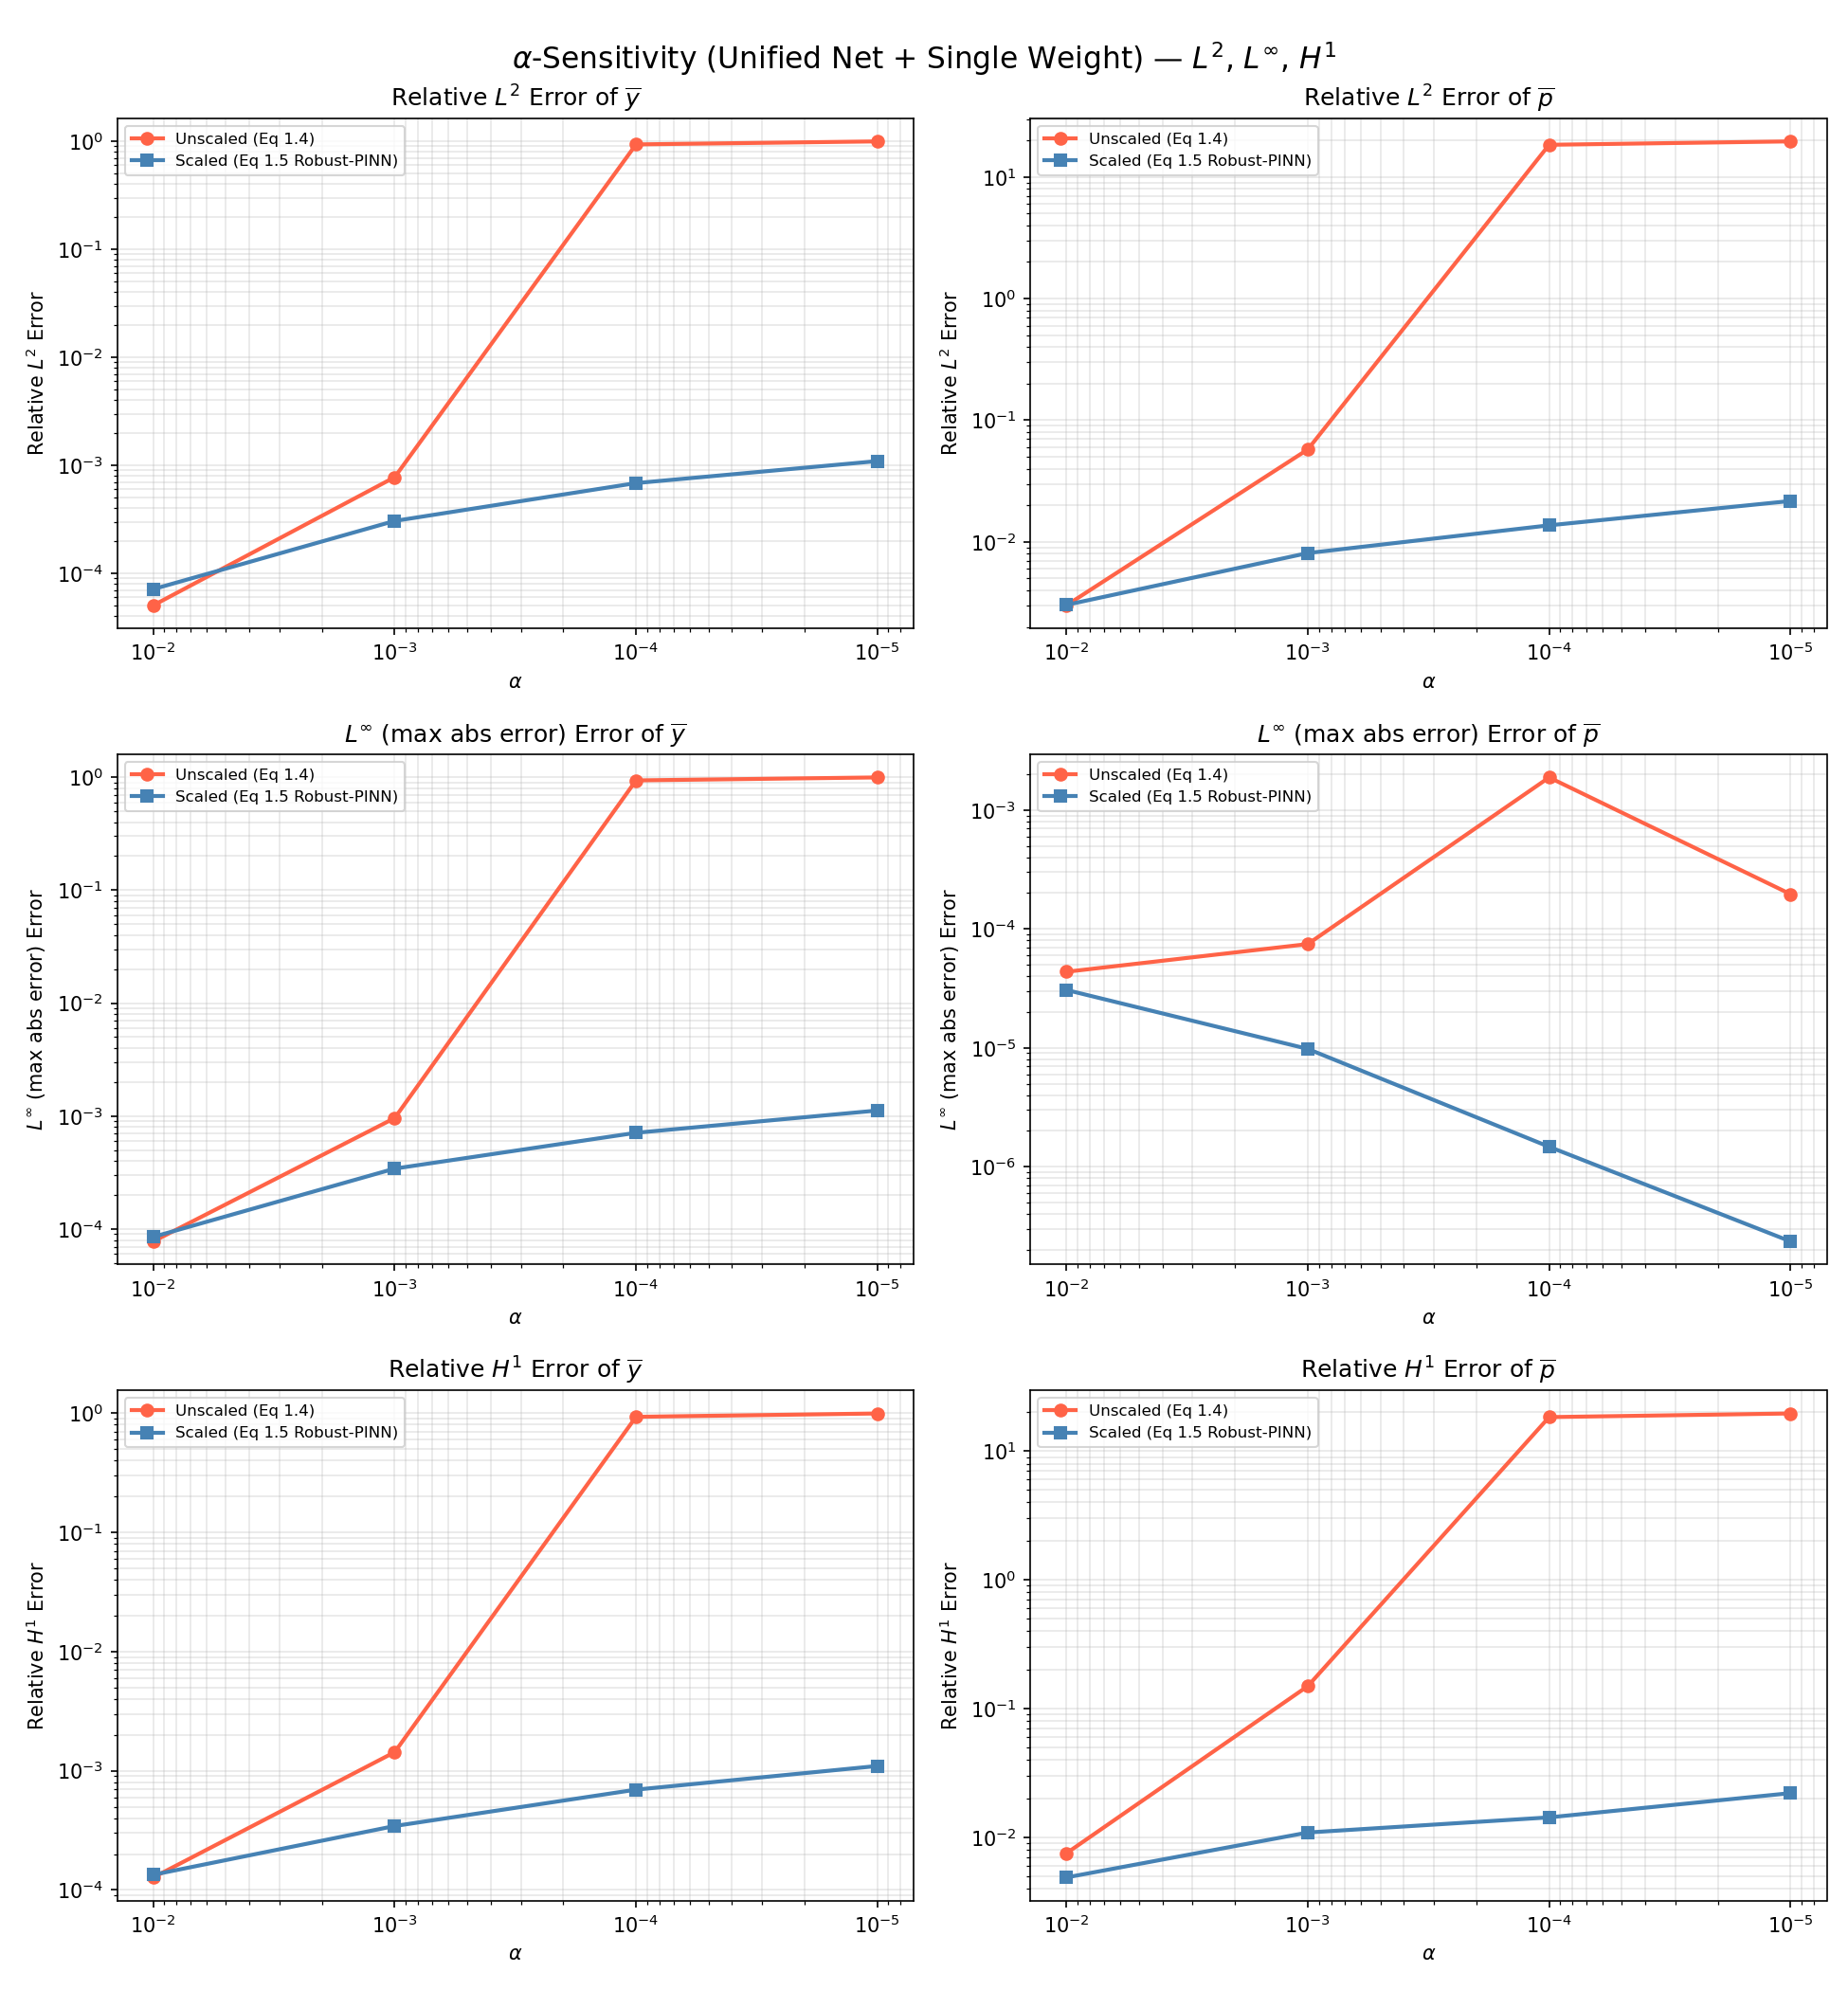
\includegraphics[width=\linewidth]{alpha_test_hardBC/unified_sensitivity_result.png}
  \caption{$\alpha$-敏感性（Hard BC + Unified Network）：
           $L^2$、$L^\infty$、$H^1$ 误差随 $\alpha$ 的变化}
  \label{fig:alpha-hard-unified}
\end{figure}




% ------------------------------------------------------------------
\subsubsection{Soft BC + Unified Network}
移除距离函数 Ansatz，改用软边界惩罚（$w_{\mathrm{bc}} = 1000$），
并在 Scaled 系统中对边界残差同样除以特征尺度进行归一化。
边界惩罚权重提升至 $w_{\mathrm{bc}} = 1000$，
$\alpha$ 的扫描范围扩展至 $\{1,\,10^{-1},\,10^{-2},\,10^{-3},\,10^{-4},\,10^{-5}\}$。

\begin{table}[H]
  \centering
  \caption{$\alpha$-敏感性实验：Soft BC + Unified Network（$w_{\mathrm{bc}}=1000$）}
  \label{tab:alpha-soft-unified}
  \small
  \begin{tabular}{cc rrrr}
    \toprule
    $\alpha$ & 系统 & $L^2_y$ & $L^2_p$ & $H^1_y$ & $H^1_p$ \\
    \midrule
    \multirow{2}{*}{$1$}
      & Unscaled & $3.57\times10^{-3}$ & $3.99\times10^{-3}$
                 & $9.72\times10^{-3}$ & $1.09\times10^{-2}$ \\
      & Scaled   & $3.81\times10^{-3}$ & $3.57\times10^{-3}$
                 & $9.23\times10^{-3}$ & $1.00\times10^{-2}$ \\
    \midrule
    \multirow{2}{*}{$10^{-1}$}
      & Unscaled & $3.45\times10^{-3}$ & $1.33\times10^{-2}$
                 & $9.69\times10^{-3}$ & $2.07\times10^{-2}$ \\
      & Scaled   & $2.51\times10^{-3}$ & $2.38\times10^{-3}$
                 & $5.37\times10^{-3}$ & $5.62\times10^{-3}$ \\
    \midrule
    \multirow{2}{*}{$10^{-2}$}
      & Unscaled & $8.39\times10^{-2}$ & $2.34\times10^{+0}$
                 & $9.23\times10^{-2}$ & $8.21\times10^{-1}$ \\
      & Scaled   & $2.15\times10^{-3}$ & $6.20\times10^{-3}$
                 & $5.35\times10^{-3}$ & $1.21\times10^{-2}$ \\
    \midrule
    \multirow{2}{*}{$10^{-3}$}
      & Unscaled & $6.00\times10^{-1}$ & $1.89\times10^{+1}$
                 & $9.54\times10^{-1}$ & $1.95\times10^{+1}$ \\
      & Scaled   & $5.79\times10^{-3}$ & $1.90\times10^{-1}$
                 & $1.12\times10^{-2}$ & $1.91\times10^{-1}$ \\
    \midrule
    \multirow{2}{*}{$10^{-4}$}
      & Unscaled & $7.03\times10^{-1}$ & $1.95\times10^{+1}$
                 & $9.86\times10^{-1}$ & $1.97\times10^{+1}$ \\
      & Scaled   & $7.23\times10^{-3}$ & $2.18\times10^{-1}$
                 & $1.27\times10^{-2}$ & $2.19\times10^{-1}$ \\
    \midrule
    \multirow{2}{*}{$10^{-5}$}
      & Unscaled & $7.15\times10^{-1}$ & $1.96\times10^{+1}$
                 & $9.87\times10^{-1}$ & $2.02\times10^{+1}$ \\
      & Scaled   & $8.81\times10^{-3}$ & $2.61\times10^{-1}$
                 & $1.41\times10^{-2}$ & $2.63\times10^{-1}$ \\
    \bottomrule
  \end{tabular}
\end{table}

\begin{figure}[H]
  \centering
  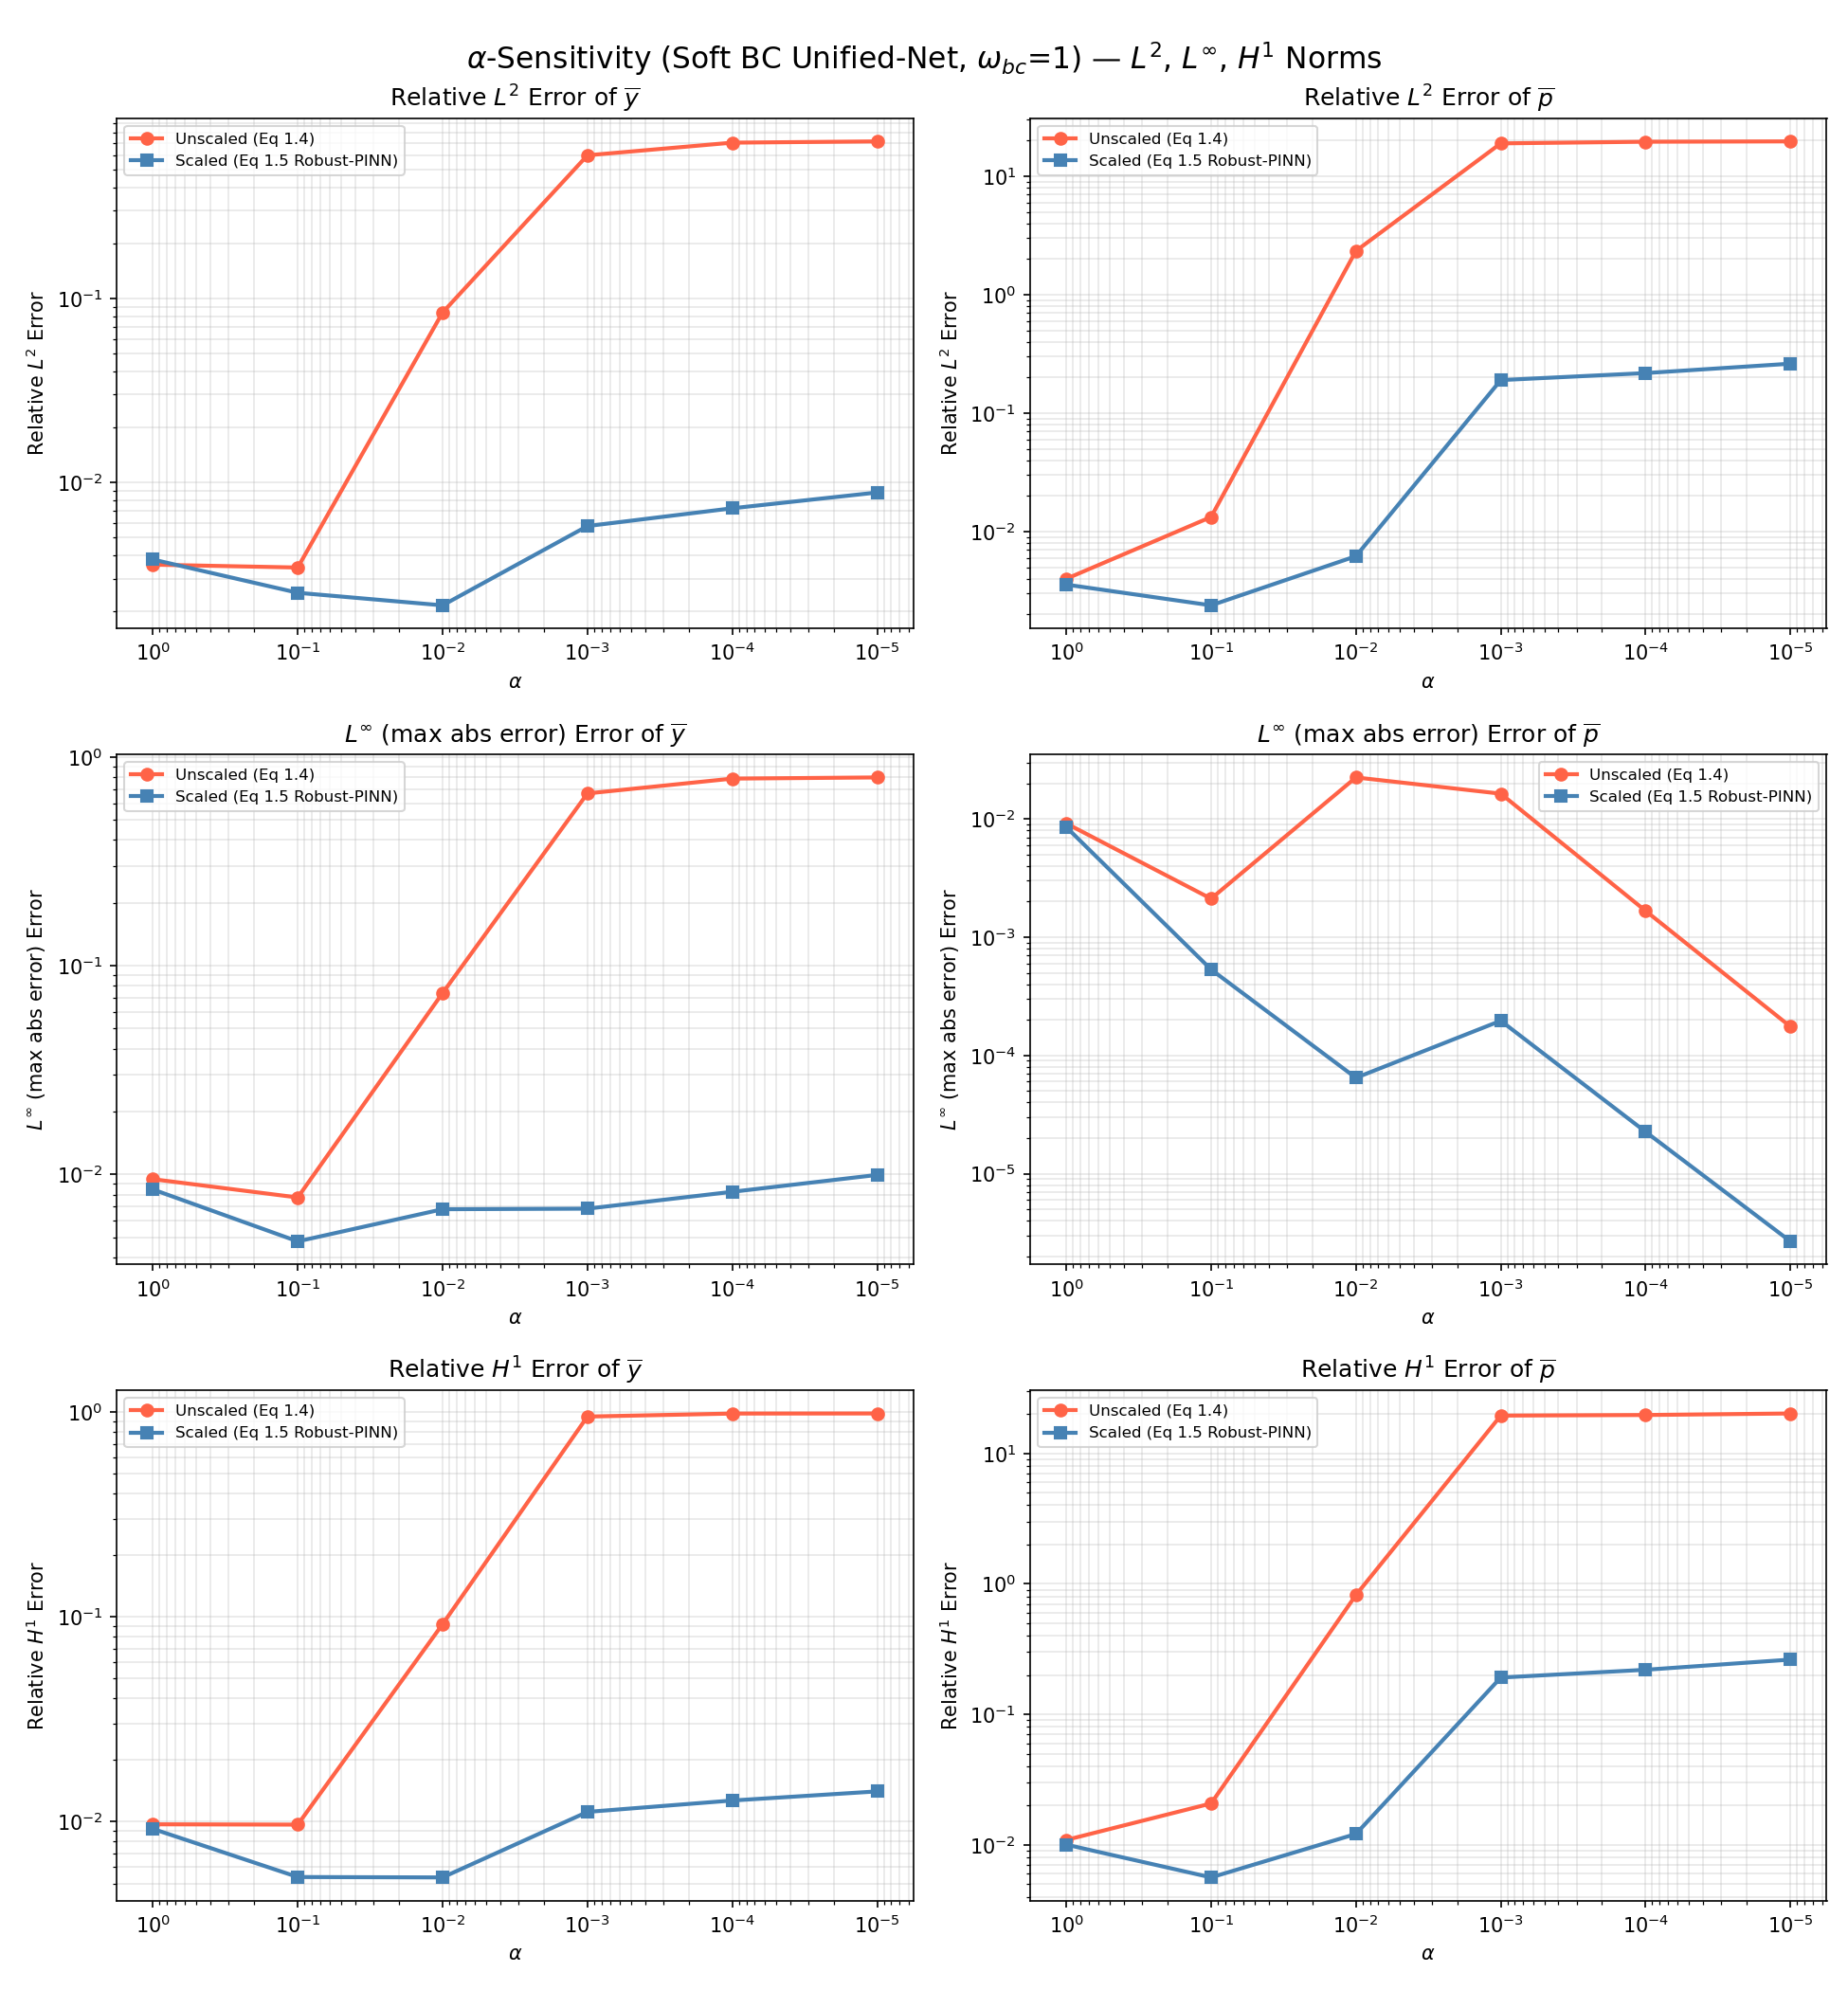
\includegraphics[width=\linewidth]{alpha_test_softBC_unified/alpha_test_softBC_unified_result1.png}
  \caption{$\alpha$-敏感性（Soft BC + Unified Network，$w_{\mathrm{bc}}=1000$）：
           $L^2$、$L^\infty$、$H^1$ 误差随 $\alpha$ 的变化}
  \label{fig:alpha-soft-unified}
\end{figure}

Scaled 系统的 $L^2_y$ 在整个 $\alpha$ 范围内稳定在 $10^{-3}$ 量级；
$L^2_p$ 降至 $\sim\!0.2$（Dual Network 下为 $\sim\!1.0$），
说明参数共享引入的隐式耦合有助于伴随状态的协同学习。
当 $\alpha \geq 10^{-2}$ 时，Scaled 的 $L^2_p$ 可降至 $10^{-3}$ 量级，
与 Hard BC 精度接近。

\textcolor{red}{问：将边界惩罚改为等权重 $w_{\mathrm{bc}} = 1$
（图~\ref{fig:alpha-soft-unified-sw}）后，
虽然Scaled 系统的 $L^2_y$ 同样保持在 $10^{-3}$--$10^{-2}$ 量级，
但Unscaled系统的误差量级也没有什么变化，且从图像上看，两条线其实几乎平行，并没有展现出hard BC时的剪刀型曲线，难以说明对于$\alpha$敏感性的降低？}

\begin{figure}[H]
  \centering
  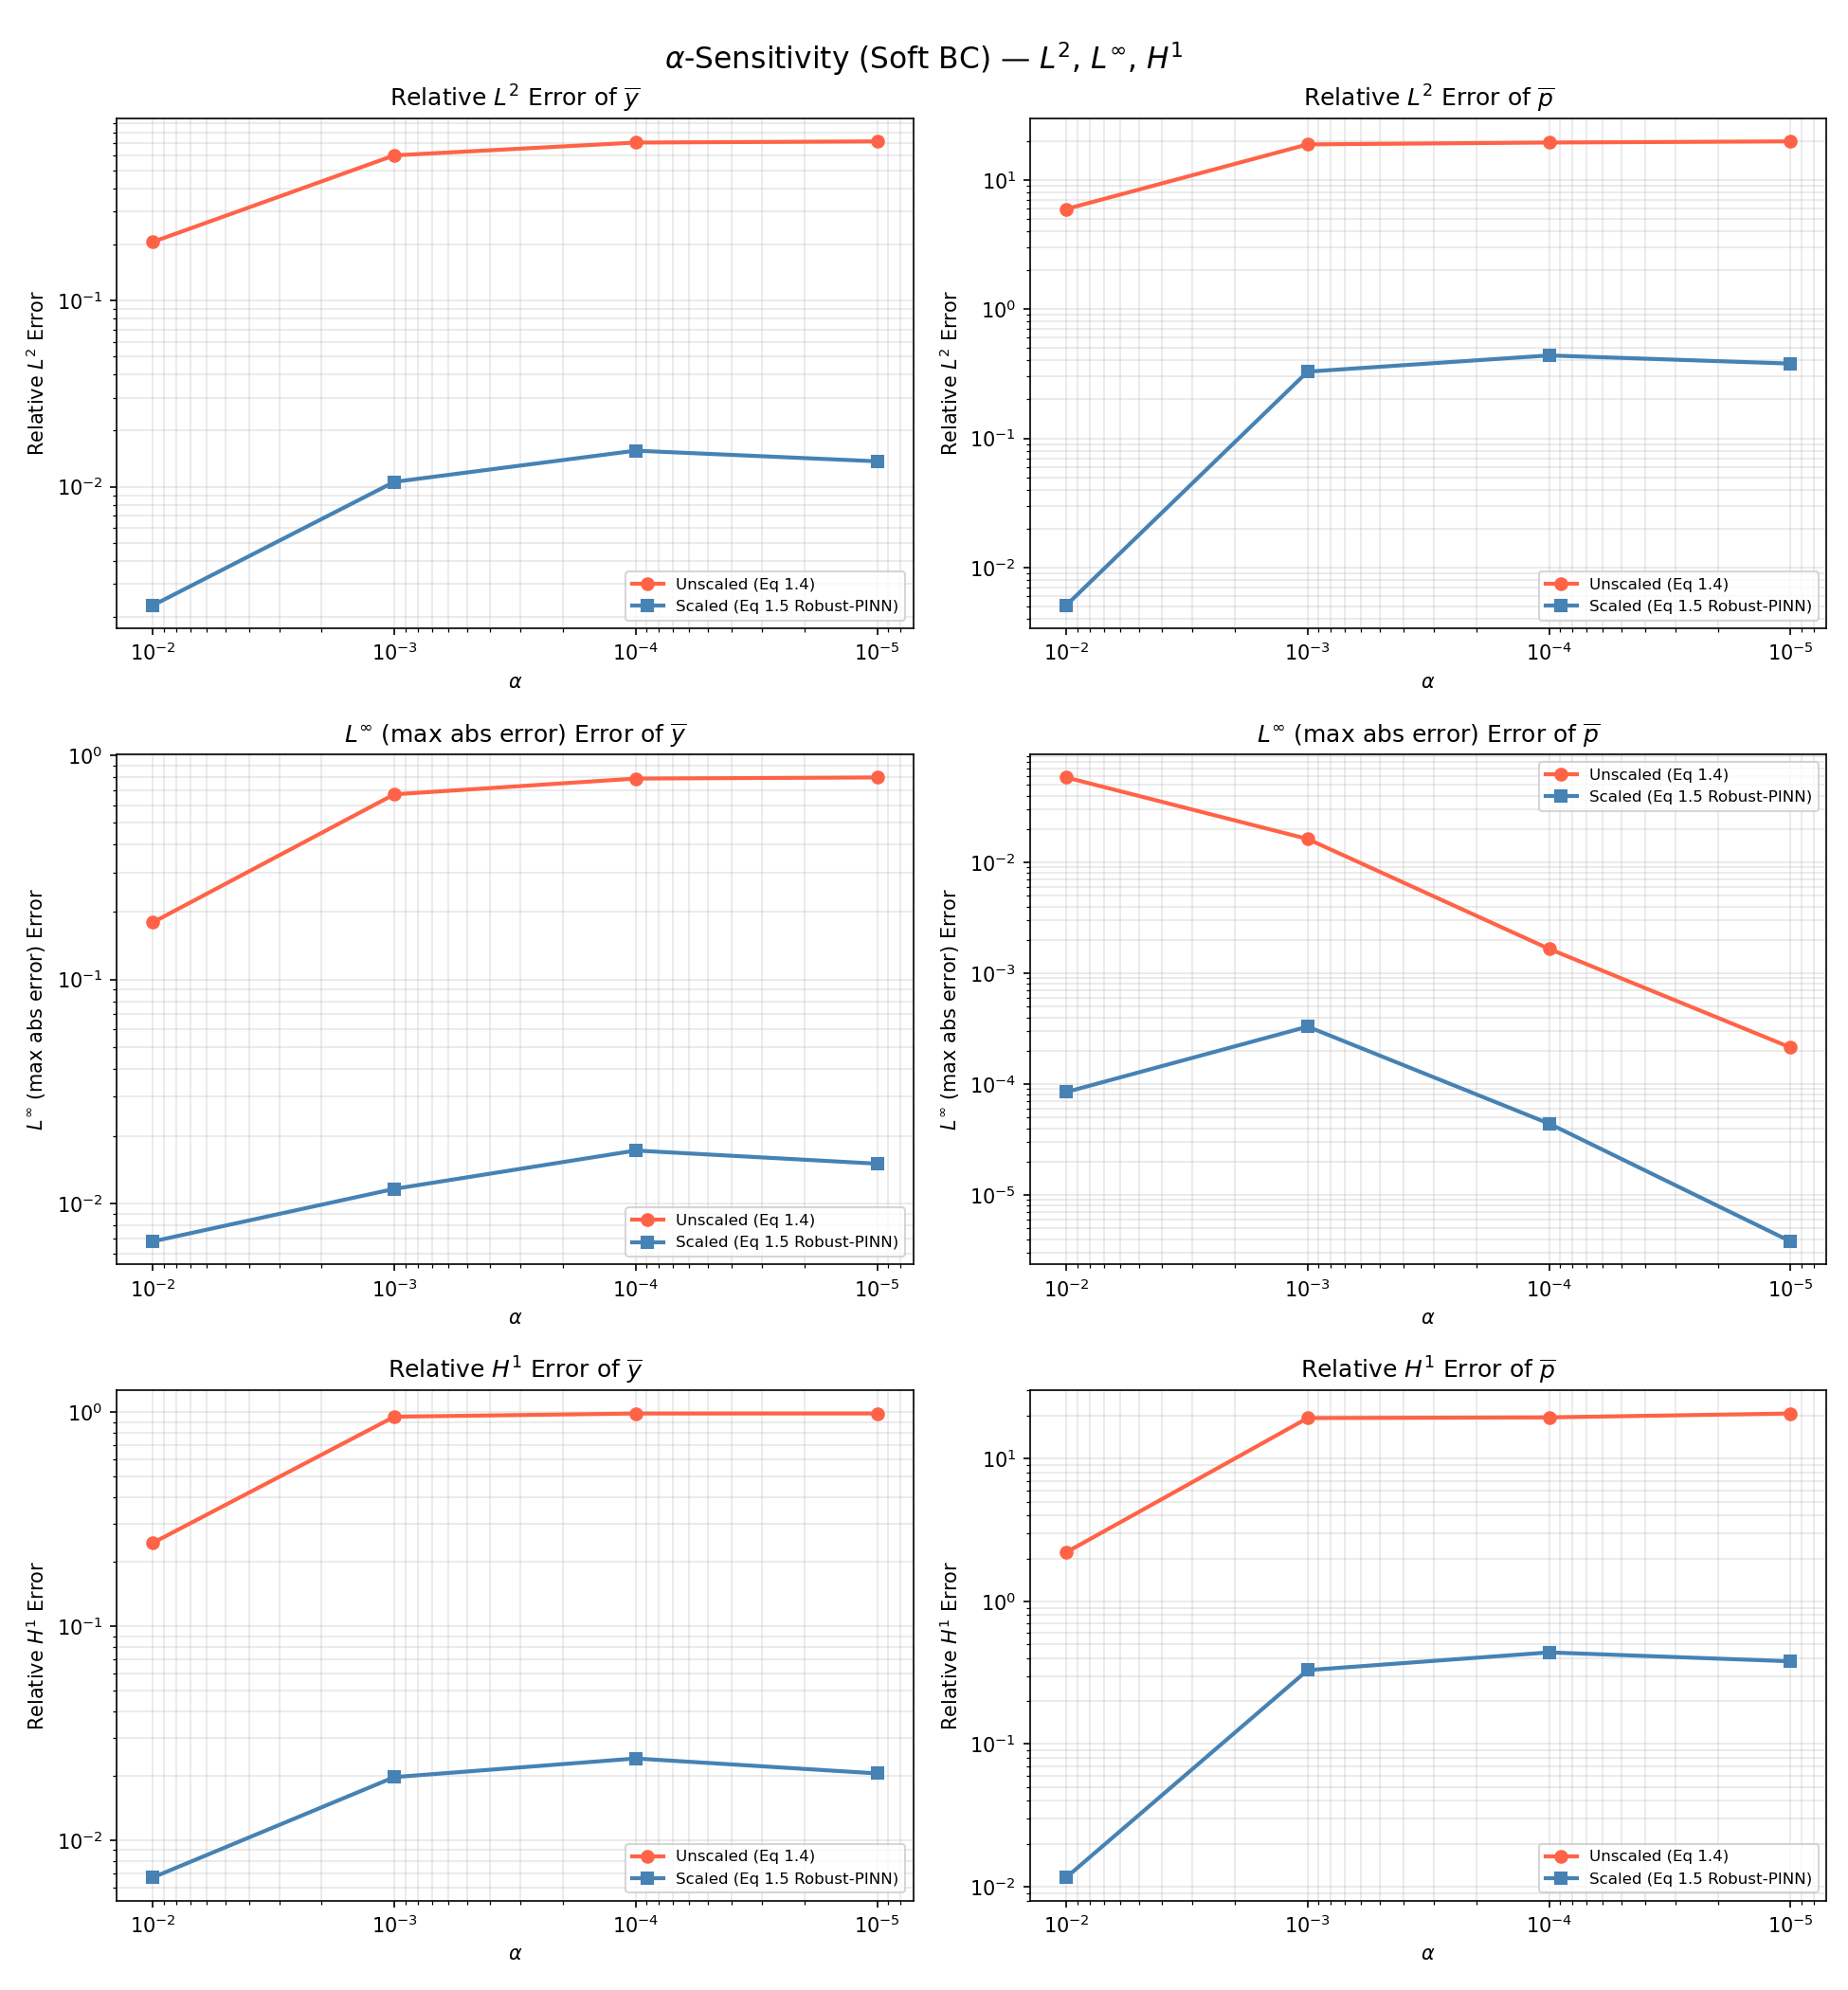
\includegraphics[width=\linewidth]{alpha_test_softBC_unified/unified_sensitivity_soft_bc_result_sameweight.png}
  \caption{Soft BC + Unified Network（等权重 $w_{\mathrm{bc}}=1$）的
           $\alpha$-敏感性对照}
  \label{fig:alpha-soft-unified-sw}
\end{figure}




% ==================================================================
\subsection{$\omega$-敏感性实验}
\label{subsec:omega-test}

固定正则化参数 $\alpha = 10^{-4}$（使系统处于高度病态状态），
敏感性实验设计了两组，2.4.1的Loss函数使用双权重，调节y和p项的权重比例，验证scaling处理之后对于Loss函数改变对error影响小
2.4.2和2.4.3则是实用单网络\\
\textcolor{red}{问：这个单网络是为了说明啥？我有点不太明白}


% ------------------------------------------------------------------
\subsubsection{Hard BC + Dual Network； Loss函数双参}

\begin{table}[H]
  \centering
  \caption{$\omega$-敏感性实验：Hard BC + Dual Network（$\alpha=10^{-4}$）}
  \label{tab:omega-hard-dual}
  \small
  \begin{tabular}{cc rrrr}
    \toprule
    $\omega$ & 系统 & $L^2_y$ & $L^2_p$ & $H^1_y$ & $H^1_p$ \\
    \midrule
    \multirow{2}{*}{$0.01$}
      & Unscaled & $3.46\times10^{-3}$ & $2.49\times10^{-1}$
                 & $6.91\times10^{-3}$ & $5.39\times10^{-1}$ \\
      & Scaled   & $1.67\times10^{-3}$ & $9.49\times10^{-2}$
                 & $2.70\times10^{-3}$ & $1.69\times10^{-1}$ \\
    \midrule
    \multirow{2}{*}{$0.1$}
      & Unscaled & $3.74\times10^{-3}$ & $2.96\times10^{-1}$
                 & $7.29\times10^{-3}$ & $6.45\times10^{-1}$ \\
      & Scaled   & $7.48\times10^{-4}$ & $6.28\times10^{-2}$
                 & $1.50\times10^{-3}$ & $1.39\times10^{-1}$ \\
    \midrule
    \multirow{2}{*}{$1$}
      & Unscaled & $1.82\times10^{-2}$ & $7.65\times10^{-1}$
                 & $2.37\times10^{-2}$ & $1.48\times10^{+0}$ \\
      & Scaled   & $1.04\times10^{-3}$ & $7.21\times10^{-2}$
                 & $1.88\times10^{-3}$ & $1.47\times10^{-1}$ \\
    \midrule
    \multirow{2}{*}{$10$}
      & Unscaled & $9.84\times10^{-1}$ & $1.94\times10^{+1}$
                 & $9.84\times10^{-1}$ & $1.94\times10^{+1}$ \\
      & Scaled   & $1.38\times10^{-3}$ & $7.04\times10^{-2}$
                 & $2.17\times10^{-3}$ & $1.18\times10^{-1}$ \\
    \midrule
    \multirow{2}{*}{$100$}
      & Unscaled & $9.90\times10^{-1}$ & $1.95\times10^{+1}$
                 & $9.90\times10^{-1}$ & $1.95\times10^{+1}$ \\
      & Scaled   & $6.67\times10^{-3}$ & $1.84\times10^{-1}$
                 & $7.44\times10^{-3}$ & $2.62\times10^{-1}$ \\
    \bottomrule
  \end{tabular}
\end{table}

Unscaled 系统在 $\omega \leq 1$ 时尚可工作但精度随 $\omega$ 增大迅速退化，
$\omega \geq 10$ 时完全崩溃（$L^2_y \approx 0.98$）；
Scaled 系统在 $\omega$ 跨越 4 个量级的范围内始终保持
$L^2_y \sim 10^{-3}$（图~\ref{fig:omega-hard-dual}）。

\begin{figure}[H]
  \centering
  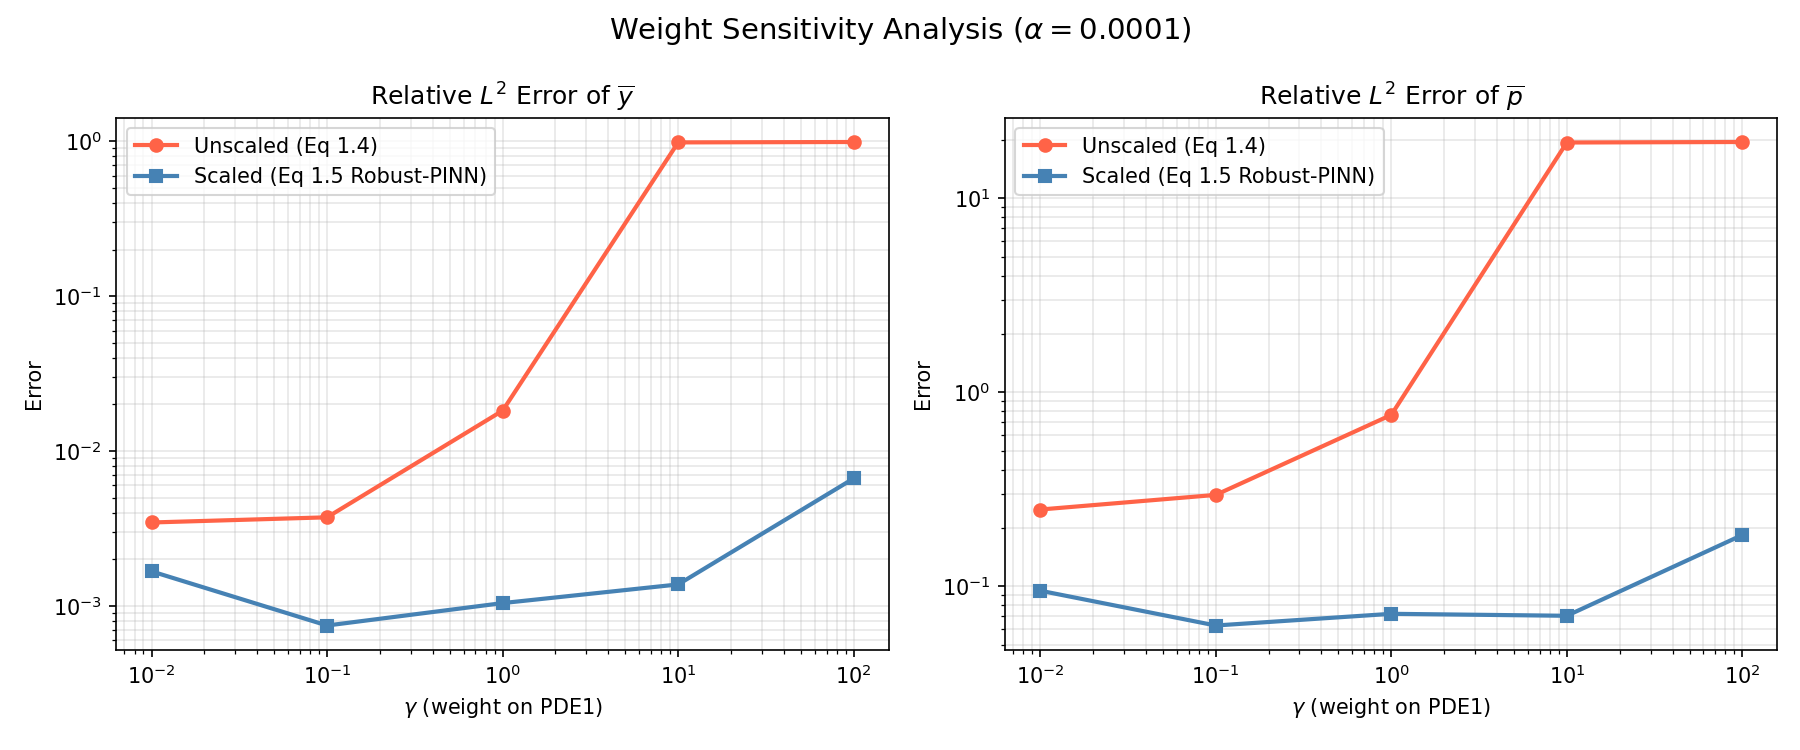
\includegraphics[width=\linewidth]{weight_test_hardBC_duelnet/weight_sensitivity_result.png}
  \caption{$\omega$-敏感性（Hard BC + Dual Network，$\alpha=10^{-4}$）：
           $L^2$、$L^\infty$、$H^1$ 误差随 $\omega$ 的变化}
  \label{fig:omega-hard-dual}
\end{figure}

Loss函数中权重的改变对于scaled系统的影响远小于unscaled系统，有效证明了scaling处理的有效性。
% ------------------------------------------------------------------
\subsubsection{Hard BC + Unified Network}

\begin{table}[H]
  \centering
  \caption{$\omega$-敏感性实验：Hard BC + Unified Network（$\alpha=10^{-4}$）}
  \label{tab:omega-hard-unified}
  \small
  \begin{tabular}{cc rrrr}
    \toprule
    $\omega$ & 系统 & $L^2_y$ & $L^2_p$ & $H^1_y$ & $H^1_p$ \\
    \midrule
    \multirow{2}{*}{$0.01$}
      & Unscaled & $9.35\times10^{-1}$ & $1.85\times10^{+1}$
                 & $9.35\times10^{-1}$ & $1.84\times10^{+1}$ \\
      & Scaled   & $2.29\times10^{-3}$ & $4.51\times10^{-2}$
                 & $2.32\times10^{-3}$ & $4.55\times10^{-2}$ \\
    \midrule
    \multirow{2}{*}{$0.1$}
      & Unscaled & $9.35\times10^{-1}$ & $1.85\times10^{+1}$
                 & $9.35\times10^{-1}$ & $1.84\times10^{+1}$ \\
      & Scaled   & $1.70\times10^{-3}$ & $3.38\times10^{-2}$
                 & $1.71\times10^{-3}$ & $3.42\times10^{-2}$ \\
    \midrule
    \multirow{2}{*}{$1$}
      & Unscaled & $9.33\times10^{-1}$ & $1.84\times10^{+1}$
                 & $9.33\times10^{-1}$ & $1.84\times10^{+1}$ \\
      & Scaled   & $6.85\times10^{-4}$ & $1.37\times10^{-2}$
                 & $6.95\times10^{-4}$ & $1.43\times10^{-2}$ \\
    \midrule
    \multirow{2}{*}{$10$}
      & Unscaled & $9.98\times10^{-1}$ & $1.97\times10^{+1}$
                 & $9.98\times10^{-1}$ & $1.97\times10^{+1}$ \\
      & Scaled   & $1.90\times10^{-4}$ & $4.57\times10^{-3}$
                 & $2.11\times10^{-4}$ & $6.48\times10^{-3}$ \\
    \midrule
    \multirow{2}{*}{$100$}
      & Unscaled & $1.13\times10^{-2}$ & $4.63\times10^{-1}$
                 & $1.48\times10^{-2}$ & $8.47\times10^{-1}$ \\
      & Scaled   & $2.84\times10^{-4}$ & $1.44\times10^{-2}$
                 & $4.47\times10^{-4}$ & $2.37\times10^{-2}$ \\
    \bottomrule
  \end{tabular}
\end{table}

Unified Network 下 Unscaled 系统在绝大多数 $\omega$ 值上均失效
（$L^2_y \approx 0.93$--$0.998$），仅在 $\omega = 100$ 时意外地部分恢复
（$L^2_y = 0.011$），说明其可用权重窗口极为狭窄且不可预测。
相比之下，Scaled 系统全程保持 $L^2_y \sim 10^{-4}$--$10^{-3}$，
且在 $\omega = 10$ 时达到最优（$L^2_y = 1.90\times10^{-4}$），
如图~\ref{fig:omega-hard-unified} 所示。

\begin{figure}[H]
  \centering
  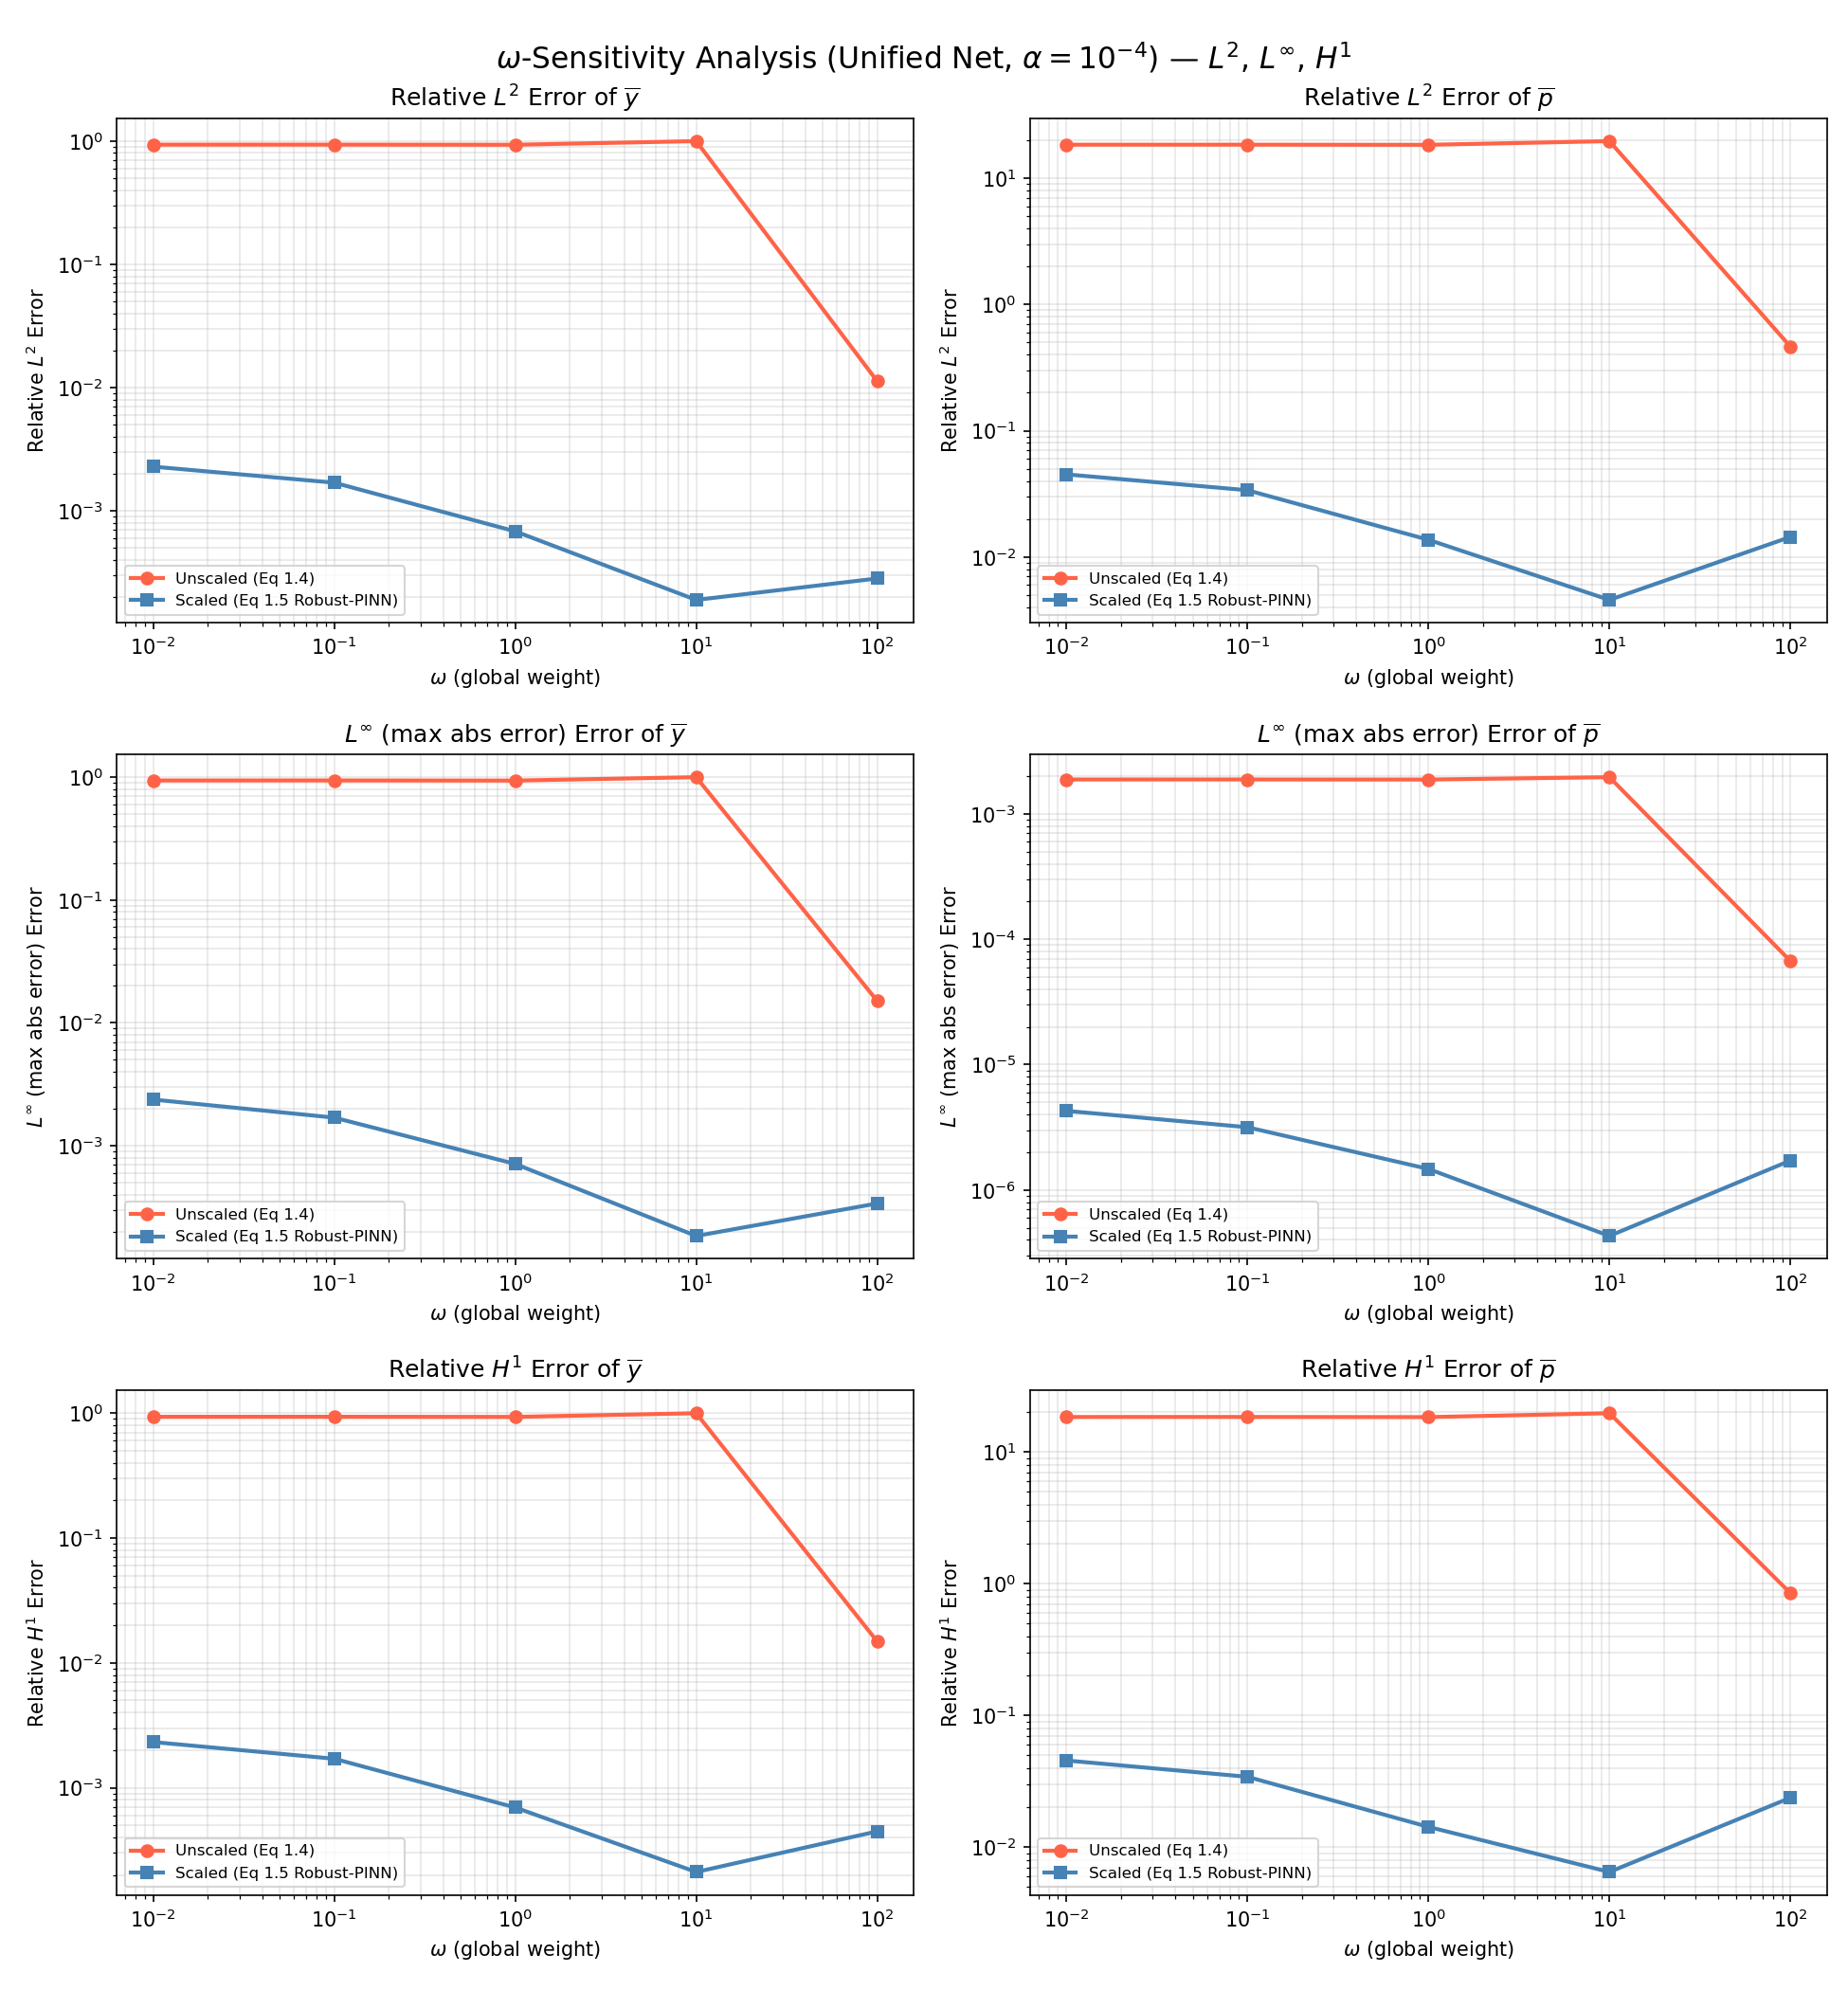
\includegraphics[width=\linewidth]{weight_test_hardBC_unified/weight_sensitivity_unified.png}
  \caption{$\omega$-敏感性（Hard BC + Unified Network，$\alpha=10^{-4}$）：
           $L^2$、$L^\infty$、$H^1$ 误差随 $\omega$ 的变化}
  \label{fig:omega-hard-unified}
\end{figure}


% ------------------------------------------------------------------
\subsubsection{Soft BC + Unified Network}

\begin{table}[H]
  \centering
  \caption{$\omega$-敏感性实验：Soft BC + Unified Network（$\alpha=10^{-4}$）}
  \label{tab:omega-soft-unified}
  \small
  \begin{tabular}{cc rrrr}
    \toprule
    $\omega$ & 系统 & $L^2_y$ & $L^2_p$ & $H^1_y$ & $H^1_p$ \\
    \midrule
    \multirow{2}{*}{$0.01$}
      & Unscaled & $9.93\times10^{-1}$ & $1.95\times10^{+1}$
                 & $9.99\times10^{-1}$ & $1.95\times10^{+1}$ \\
      & Scaled   & $4.21\times10^{-2}$ & $8.37\times10^{-1}$
                 & $4.25\times10^{-2}$ & $8.37\times10^{-1}$ \\
    \midrule
    \multirow{2}{*}{$0.1$}
      & Unscaled & $9.38\times10^{-1}$ & $1.94\times10^{+1}$
                 & $9.96\times10^{-1}$ & $1.94\times10^{+1}$ \\
      & Scaled   & $3.72\times10^{-2}$ & $7.83\times10^{-1}$
                 & $3.99\times10^{-2}$ & $7.83\times10^{-1}$ \\
    \midrule
    \multirow{2}{*}{$1$}
      & Unscaled & $7.05\times10^{-1}$ & $1.94\times10^{+1}$
                 & $9.87\times10^{-1}$ & $1.95\times10^{+1}$ \\
      & Scaled   & $1.56\times10^{-2}$ & $4.38\times10^{-1}$
                 & $2.41\times10^{-2}$ & $4.39\times10^{-1}$ \\
    \midrule
    \multirow{2}{*}{$10$}
      & Unscaled & $5.96\times10^{-1}$ & $1.93\times10^{+1}$
                 & $9.83\times10^{-1}$ & $1.91\times10^{+1}$ \\
      & Scaled   & $2.10\times10^{-2}$ & $7.37\times10^{-1}$
                 & $4.25\times10^{-2}$ & $7.45\times10^{-1}$ \\
    \midrule
    \multirow{2}{*}{$100$}
      & Unscaled & $6.12\times10^{-1}$ & $1.98\times10^{+1}$
                 & $9.94\times10^{-1}$ & $2.05\times10^{+1}$ \\
      & Scaled   & $1.15\times10^{-2}$ & $4.00\times10^{-1}$
                 & $2.26\times10^{-2}$ & $4.56\times10^{-1}$ \\
    \bottomrule
  \end{tabular}
\end{table}

软边界下 Unscaled 的 $L^2_y$ 在 $0.59$--$0.99$ 之间剧烈波动，
$L^2_p$ 始终 $\approx 19$（完全未学到 $\bar{p}$）；
Scaled 的 $L^2_y$ 稳定在 $0.01$--$0.04$，
在所有 $\omega$ 下均保持 $1$--$2$ 个量级的显著优势
（图~\ref{fig:omega-soft-unified}）。

\begin{figure}[H]
  \centering
  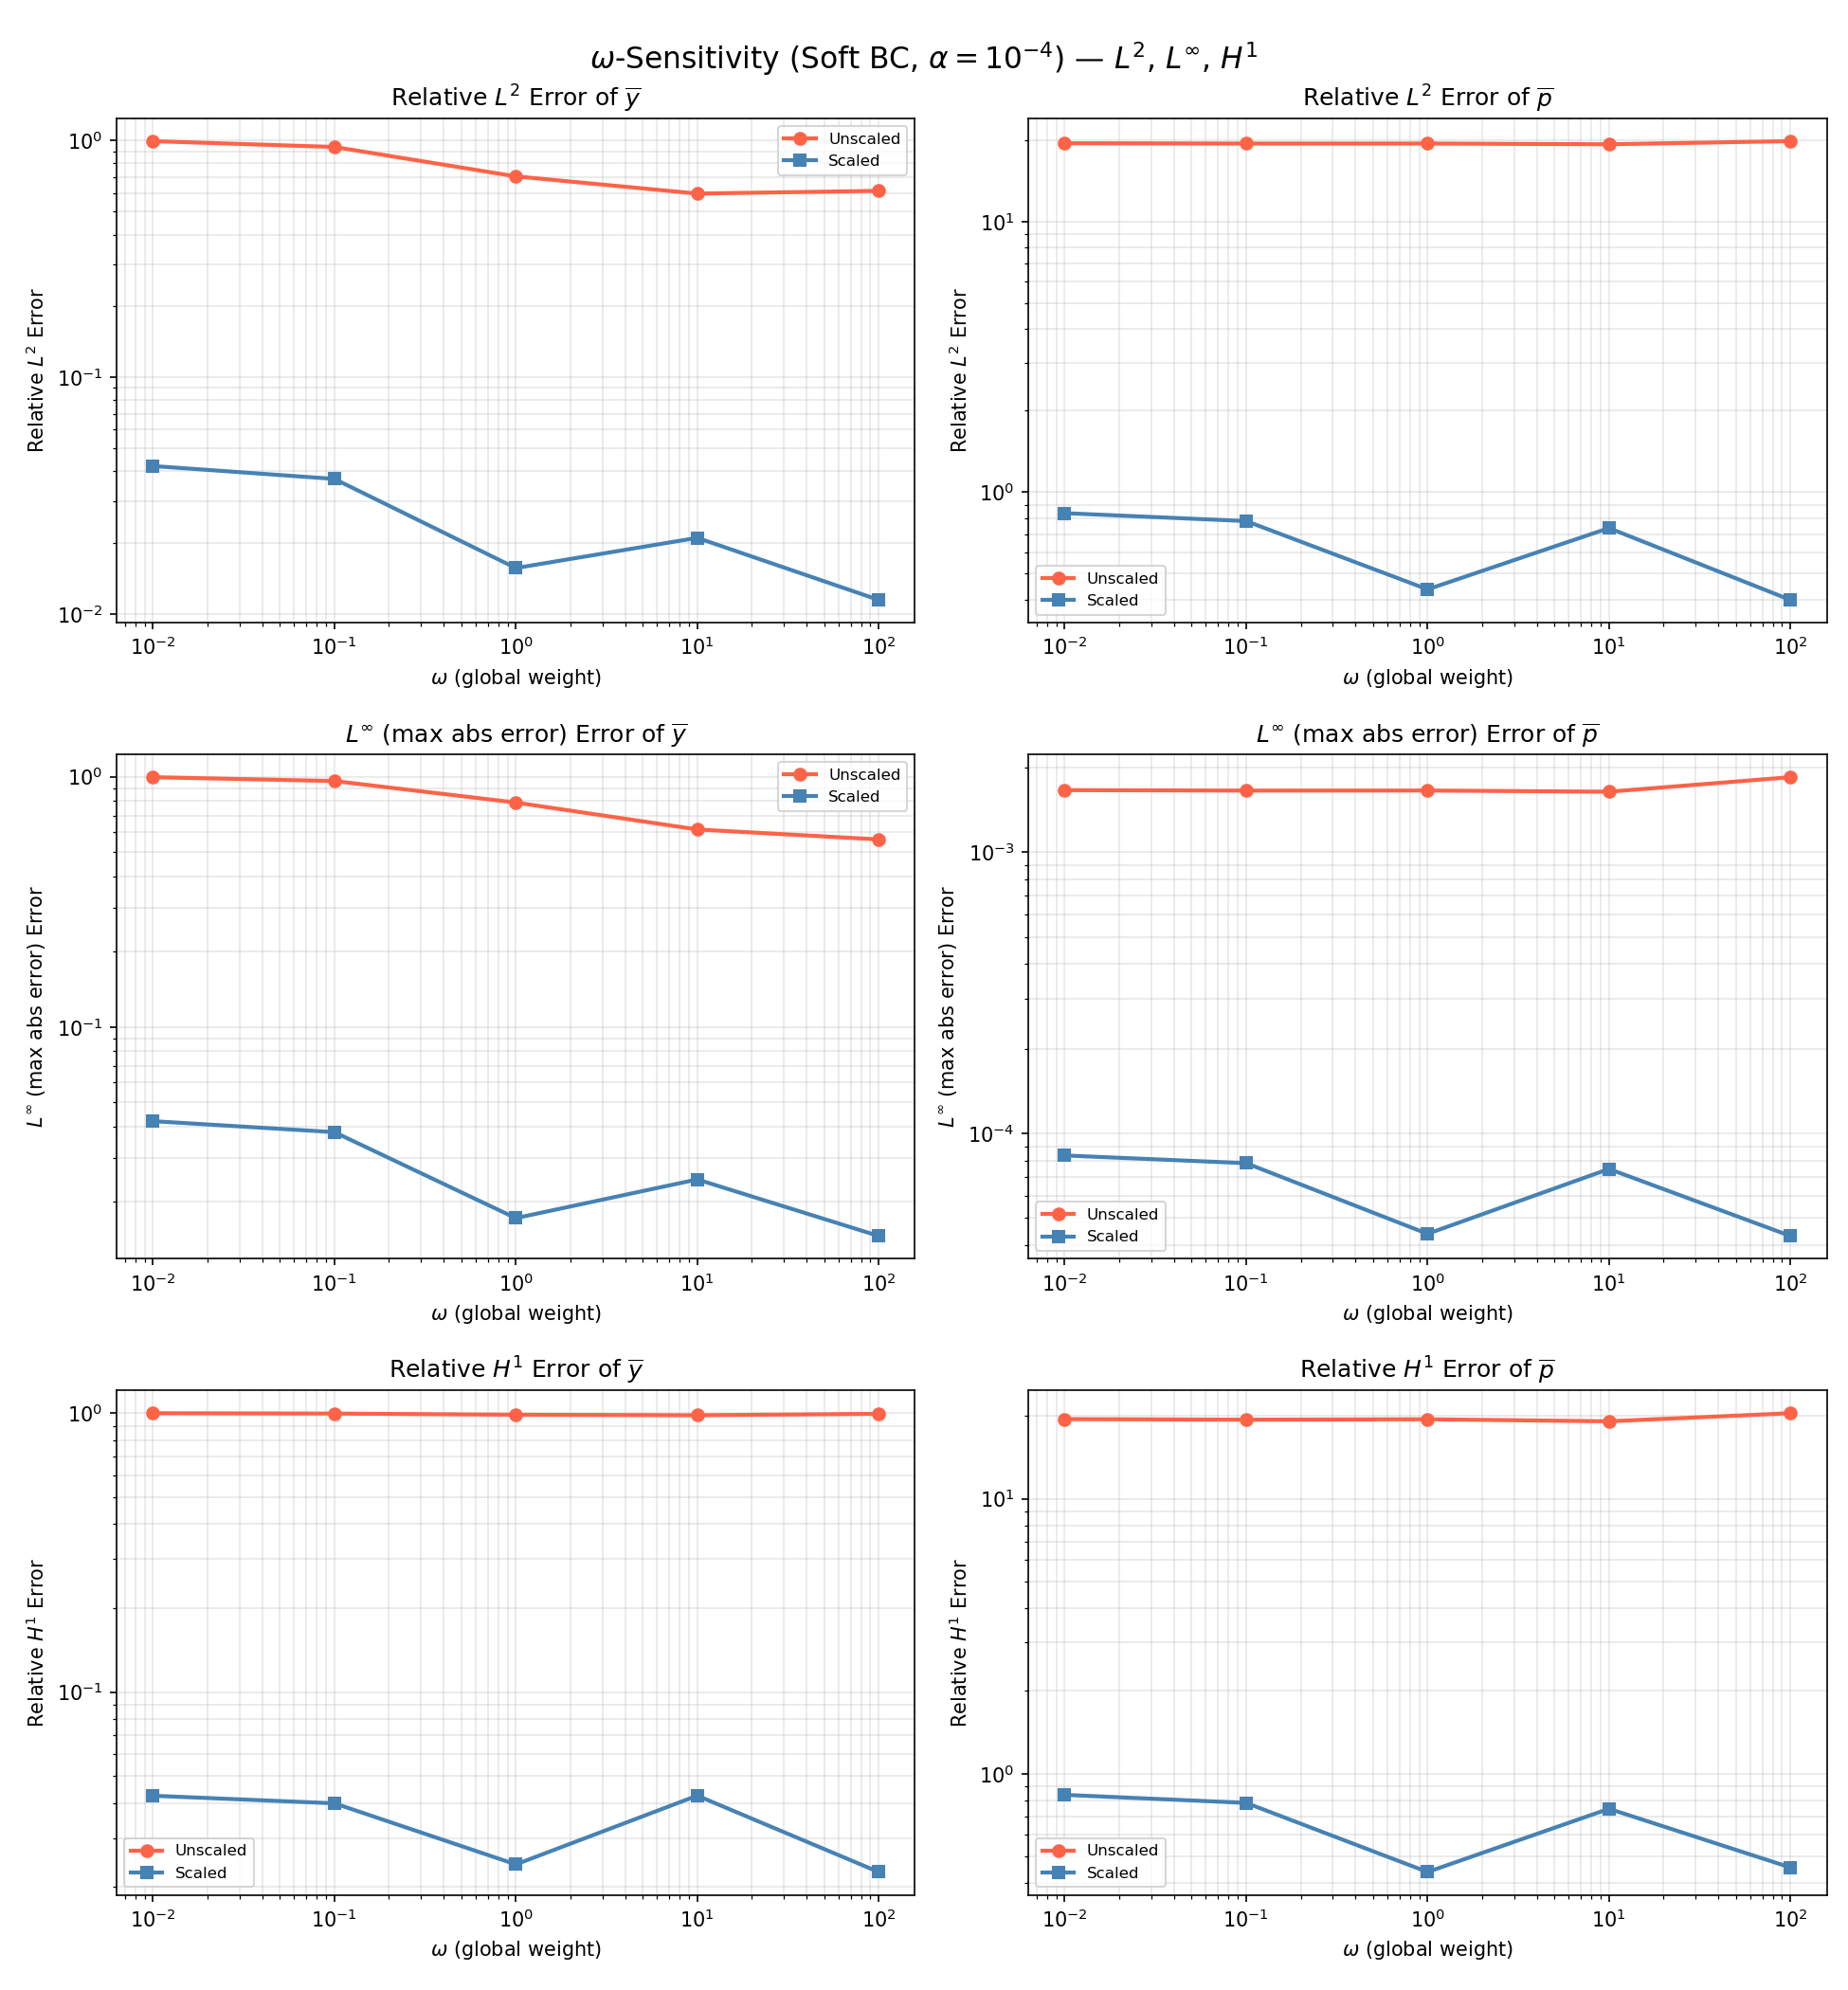
\includegraphics[width=\linewidth]{weight_test_softBC_unified/weight_sensitivity_soft_bc.png}
  \caption{$\omega$-敏感性（Soft BC + Unified Network，$\alpha=10^{-4}$）：
           $L^2$、$L^\infty$、$H^1$ 误差随 $\omega$ 的变化}
  \label{fig:omega-soft-unified}
\end{figure}




% ==================================================================
\subsection{综合分析}
\label{subsec:synthesis}

\paragraph{Hard BC vs.\ Soft BC。}
Hard BC 通过距离函数 Ansatz 精确满足边界条件，使网络仅需优化内部 PDE 残差，
是 Scaling 效果最理想的场景（$L^2 \sim 10^{-4}$）。
Soft BC 引入了边界与内部残差的竞争，绝对精度降低约 $1$--$2$ 个量级
（$L^2 \sim 10^{-2}$），但 Scaling 的相对优势依然显著。
在实际应用中，复杂几何往往使 Hard BC 不可用，
而 Soft BC + Scaling + 边界归一化的组合仍能保证数量级的改进。


\paragraph{不同范数的表现。}
\begin{itemize}

    \item{$L_2$和$L_{H_1}$十分相似的原因:}\\
    在 PINN 的训练中，网络通常能很好地学到解，但往往会在振幅上产生微小的偏差。假设网络的预测值只在振幅上差了一个极小的比例 $\epsilon$:
    \begin{equation}
        y_{pred}(x) \approx (1 - \epsilon) y_{exact}(x) 
    \end{equation}

那么，误差函数 $e(x)$ 就完全正比于精确解本身：
\begin{equation}
    e(x) = y_{pred}(x) - y_{exact}(x) = -\epsilon \cdot y_{exact}(x)
\end{equation} 

同理，误差的梯度也正比于精确解的梯度：
\begin{equation}
    \nabla e(x) = -\epsilon \cdot \nabla y_{exact}(x)
\end{equation}

带入$L_2$ 误差：
\begin{equation}
    \text{Error}_{L^2} = \sqrt{\frac{\|e\|_{L^2}^2}{\|y_{exact}\|_{L^2}^2}} = \sqrt{\frac{(-\epsilon)^2 \|y_{exact}\|_{L^2}^2}{\|y_{exact}\|_{L^2}^2}} = \epsilon
\end{equation} 

带入$L_{H^1}$ 误差：
\begin{align}
    \text{Error}_{H^1} &= \sqrt{\frac{\|e\|_{L^2}^2 + \|\nabla e\|_{L^2}^2}{\|y_{exact}\|_{L^2}^2 + \|\nabla y_{exact}\|_{L^2}^2}}\\
    &= \sqrt{\frac{\epsilon^2 \left( \|y_{exact}\|_{L^2}^2 + \|\nabla y_{exact}\|_{L^2}^2 \right)}{\|y_{exact}\|_{L^2}^2 + \|\nabla y_{exact}\|_{L^2}^2}}  (\|e\|^2 = \epsilon^2 \|y_{exact}\|^2;\|\nabla e\|^2 = \epsilon^2 \|\nabla y_{exact}\|^2)\\
    &= \sqrt{\epsilon^2} = \epsilon
\end{align}
因此，在学习良好的数值试验中，$L_2$和$L_{H_1}$的值几乎相同\\

事实上，$L_2$和$L_{H_1}$之间受着更为深远的数学性质的制约。在偏微分方程的Sobolev空间理论中，根据椭圆正则性定理，即：对于泊松方程 $-\Delta e = r$（其中 $r$ 是残差），存在一个常数 $C_1$，使得：$$ \|e\|_{H^2} \le C_1 \|r\|_{L^2} $$这意味着，只要 PINN 把 PDE 的残差降下来了，误差的二阶导数就被强行界定住了。

\item{$L_\infty$范数的不同表现：}\\
对于无穷范数来说，与另外两种全局的相对范数不同，它是一种由局部极值所决定的最大值范数，因此表现不同。


\end{itemize}




% ==================================================================
\subsection{数学证明}
\label{subsec:math-defs}

式 (1.5) 为缩放后的一阶最优性系统：
\begin{equation}
\begin{cases}
-\alpha^{1/2}\Delta y + p = \alpha^{3/4}(f+u_d) & \text{in } \Omega \\
-\alpha^{1/2}\Delta p - y = -\alpha^{1/4}y_d & \text{in } \Omega
\end{cases}
\end{equation}
并伴随齐次 Dirichlet 边界条件 $y=0, p=0$ on $\partial\Omega$。

利用测试函数 $w \in H_0^1(\Omega)$，$v \in H_0^1(\Omega)$ 构建等价的弱形式系统：
\begin{equation}
\begin{cases}
\alpha^{1/2}(\nabla p, \nabla w) - (y, w) &= -\alpha^{1/4}(y_d, w) \quad \forall w \in H_0^1(\Omega) \\
(p, v) + \alpha^{1/2}(\nabla y, \nabla v) &= \alpha^{3/4}(f+u_d, v) \quad \forall v \in H_0^1(\Omega)
\end{cases}
\end{equation}
最优控制问题的一阶必要条件是由关于 $y$的状态方程和关于 $p$的伴随状态方程组成的一个相互耦合的系统。为了对其进行整体的泛函分析，引入联合解空间 $V := (H_\alpha^1(\Omega))^2$ 和联合测试函数 $(w, v)$，将这两个方程的弱形式叠加，构造出了一个紧凑的$H_{0}^{1}(\Omega)\times H_{0}^{1}(\Omega)$ 上的全局双线性形式 $\mathcal{K}((y, p), (w, v))$，其中

\begin{equation}
    \begin{cases}
        \mathcal{K}((y,p),(w,v))&:=\alpha^{1/2}a(w,p)-(y,w)+(p,v)+\alpha^{1/2}a(y,v)\\
        g(w,v)&:=-\alpha^{1/4}(y_{d},w)+\alpha^{3/4}(f+u_{d},v)
    \end{cases}
\end{equation}

（注：$a(v,w):=\int_{\Omega}\nabla v\cdot\nabla w~dx$  $\forall v,w\in H_{0}^{1}(\Omega)$）



这种构造的依据是将复杂的耦合 PDE 问题转化为一个标准的单一变分问题：
\begin{equation}
    \mathcal{K}((y, p), (w, v)) = g(w, v)
\end{equation}
其中，通过这种紧凑的表达方式，可以更直接地应用inf-sup 理论来证明这一鞍点问题的稳定性以及统一变量$y$与$p$的解空间。


为了衡量误差和系统的稳定性，我们定义依赖于参数 $\alpha$ 的加权能量范数 $H_\alpha^1(\Omega)$：
\begin{equation}
\|v\|_{H_\alpha^1(\Omega)} := \left( \|v\|_{L^2(\Omega)}^2 + \alpha^{1/2}\|\nabla v\|_{L^2(\Omega)}^2 \right)^{1/2}
\end{equation}
并且将在乘积空间 $V$ 上的组合范数定义为：
\begin{equation}
\|(y,p)\|_V := \left( \|y\|_{H_\alpha^1(\Omega)}^2 + \|p\|_{H_\alpha^1(\Omega)}^2 \right)^{1/2}
\end{equation}


\begin{lemma}
对于由式 (1.5) 导出的双线性形式 $\mathcal{K}(\cdot, \cdot)$，存在独立于 $\alpha$ 的正常数 $c_0$ 和 $C_1$，使得：
\begin{equation}
c_0 \|(y,p)\|_V \le \sup_{(w,v)\in V} \frac{\mathcal{K}((y,p),(w,v))}{\|(w,v)\|_V} \le C_1 \|(y,p)\|_V
\end{equation}
\end{lemma}

\begin{proof}
\textbf{(1) 证明双线性形式的连续性（上限 $C_1$）：}

利用柯西-施瓦茨不等式（Cauchy-Schwarz inequality），我们对双线性形式的绝对值进行放缩：
\begin{align*}
\mathcal{K}((y,p), (w,v)) 
&=\alpha^{1/2}a(w,p)-(y,w)+(p,v)+\alpha^{1/2}a(y,v)\\
&\le \|y\|_{L^2} \|w\|_{L^2} + \alpha^{1/2}\|\nabla p\|_{L^2} \|\nabla w\|_{L^2} + \|p\|_{L^2} \|v\|_{L^2} + \alpha^{1/2}\|\nabla y\|_{L^2} \|\nabla v\|_{L^2}
\end{align*}
应用离散的柯西-施瓦茨不等式 $\sum a_i b_i \le \sqrt{\sum a_i^2}\sqrt{\sum b_i^2}$，可得：
\begin{align*}
\mathcal{K}((y,p), (w,v)) &\le \left(\|y\|_{L^2}^2 + \alpha^{1/2}\|\nabla y\|_{L^2}^2 + \|p\|_{L^2}^2 + \alpha^{1/2}\|\nabla p\|_{L^2}^2 \right)^{1/2} \\
&\quad \cdot \left(\|w\|_{L^2}^2 + \alpha^{1/2}\|\nabla w\|_{L^2}^2 + \|v\|_{L^2}^2 + \alpha^{1/2}\|\nabla v\|_{L^2}^2 \right)^{1/2}
\end{align*}
化简后即为：
\begin{equation}
\mathcal{K}((y,p), (w,v)) \le \|(y,p)\|_V \cdot \|(w,v)\|_V
\end{equation}
这证明了连续性，且上限常数 $C_1 = 1$。

\medskip
\textbf{(2) 证明 inf-sup 下界稳定性条件（下限 $c_0$）：}

为证明$c_0 \|(y,p)\|_V \le \sup_{(w,v)\in V} \frac{\mathcal{K}((y,p),(w,v))}{\|(w,v)\|_V}$，即证明存在测试函数$w_0$,$v_0$使得存在$c_0 \|(y,p)\|_V \le  \frac{\mathcal{K}((y,p),(w_0,v_0))}{\|(w_0,v_0)\|_V}$。\\
则对于任意给定的 $(y,p) \in V$，构造特定的测试函数：令 $w = p - y$ 以及 $v = p + y$。\\
代入双线性形式展开：
\begin{align*}
\mathcal{K}((y,p), (p-y, p+y)) &= \alpha^{1/2}(\nabla p, \nabla(p-y)) - (y, p-y) + (p, p+y) + \alpha^{1/2}(\nabla y, \nabla(p+y)) \\
&= \alpha^{1/2}(\nabla p, \nabla p) - \alpha^{1/2}(\nabla p, \nabla y) - (y,p) + (y,y) + (p,p) + (p,y) \\
&\quad + \alpha^{1/2}(\nabla y, \nabla p) + \alpha^{1/2}(\nabla y, \nabla y)\\
&=(y,y)+ \alpha^{1/2}(\nabla y, \nabla y) + (p,p)+ \alpha^{1/2}(\nabla p, \nabla p)\\
&=\|y\|_{L^2}^2 + \alpha^{1/2}\|\nabla y\|_{L^2}^2 + \|p\|_{L^2}^2 + \alpha^{1/2}\|\nabla p\|_{L^2}^2 \\
&= \|(y,p)\|_V^2
\end{align*}

计算构造的测试函数范数，由平行四边形法则知:
\begin{align}
\|(w,v)\|_V^2 
&= \|p-y\|_{H_\alpha^1}^2 + \|p+y\|_{H_\alpha^1}^2 \\
&= \|p\|_{H_\alpha^1}^2 + \|y\|_{H_\alpha^1}^2
\end{align}

由此可得：
\begin{equation}
\frac{\mathcal{K}((y,p), (w,v))}{\|(w,v)\|_V} = \frac{\|(y,p)\|_V^2}{\sqrt{2}\|(y,p)\|_V} = \frac{1}{\sqrt{2}}\|(y,p)\|_V
\end{equation}
因此：
\begin{equation}
\sup_{(w,v)\in V} \frac{\mathcal{K}((y,p), (w,v))}{\|(w,v)\|_V} \ge \frac{1}{\sqrt{2}} \|(y,p)\|_V
\end{equation}
即下界常数 $c_0 = 1/\sqrt{2}$，证明完毕。
\end{proof}
该引理的证明对于使用物理信息神经网络（PINNs）求解最优控制问题具有决定性的理论指导和算法稳定意义：
\begin{itemize}
    \item 从数学底层消除神经网络训练的“梯度病态”\\
    PINN 的训练过程高度依赖于基于梯度的优化器（本实验中为Adam 及 L-BFGS）来更新网络权重。如果底层的 PDE 系统本身条件数很差（随 $\alpha$→0 爆炸），损失函数的优化地貌将变得极度扭曲，容易导致梯度崩溃或陷入不良的局部最优。而本引理严格证明了该缩放系统在加权范数下，其双线性形式的连续性上界 $C_1$和 inf-sup 稳定性下界$c_0$是完全独立于$\alpha$的。这相当于在连续层面上对物理方程进行了理想的“预处理”，从根本上解耦了系统条件数与$\alpha$的联系，保证了神经网络在计算损失函数梯度时不会因为极小的$\alpha$而引发数值不稳定。
    \item 为设计“Robust-PINN”提供严密的理论背书\\
    正是因为直接用 PINN 求解原始问题存在不稳定性，我们需要一套在理论上无懈可击的新系统来设计算法。本引理证明了缩放后的系统在解空间及其对偶空间之间诱导了一个独立于参数$\alpha$的同构关系。这一泛函分析层面的强有力结论保证了：无论正则化参数多么微小，该系统都不会发生算子退化。这直接促成了鲁棒物理信息神经网络（Robust-PINN）的提出，使得深度学习求解器能够真正胜任惩罚参数极小的复杂最优控制问题。
    \item 统一变量解空间，简化网络架构与权重设计\\
    在应用 PINN 求解最优控制问题时，神经网络通常需要同时输出状态变量 $y$ 和伴随状态变量 $p$。未缩放时，它们的自然范数是不同的（分别带有 $\alpha^{1/2}$ 和 $\alpha^{-1/2}$ 权重）。而本引理证明了经过缩放后，不仅 $y$ 和 $p$ 可以存在于同一个解空间 $V = (H_\alpha^1(\Omega))^2$ 中，而且它们可以完美地共享同一个加权能量范数 $\|(y,p)\|_V$。故而对于 PINN 的实施而言，这意味着神经网络的多个输出在物理量纲和误差尺度上已经达到了天然对齐，从而避免了在损失函数中人工盲目调节不同物理量残差权重的繁琐工作


\end{itemize}

% ==================================================================
\section{Part 1 解法说明}
\label{sec:part1}

\begin{figure}[H]
  \centering
  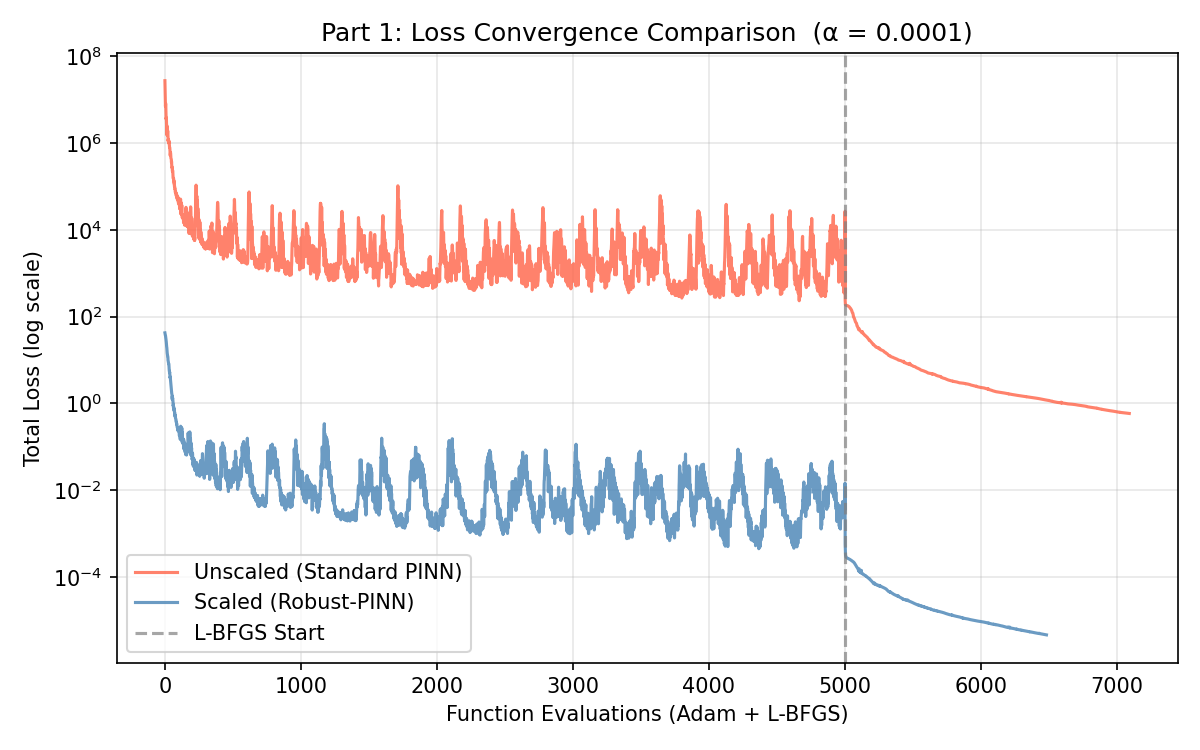
\includegraphics[width=0.85\linewidth]{part1_loss_comparison_20260301_091035.png}
  \caption{Part 1 各损失分量演化曲线}
  \label{fig:loss}
\end{figure}

\begin{figure}[H]
  \centering
  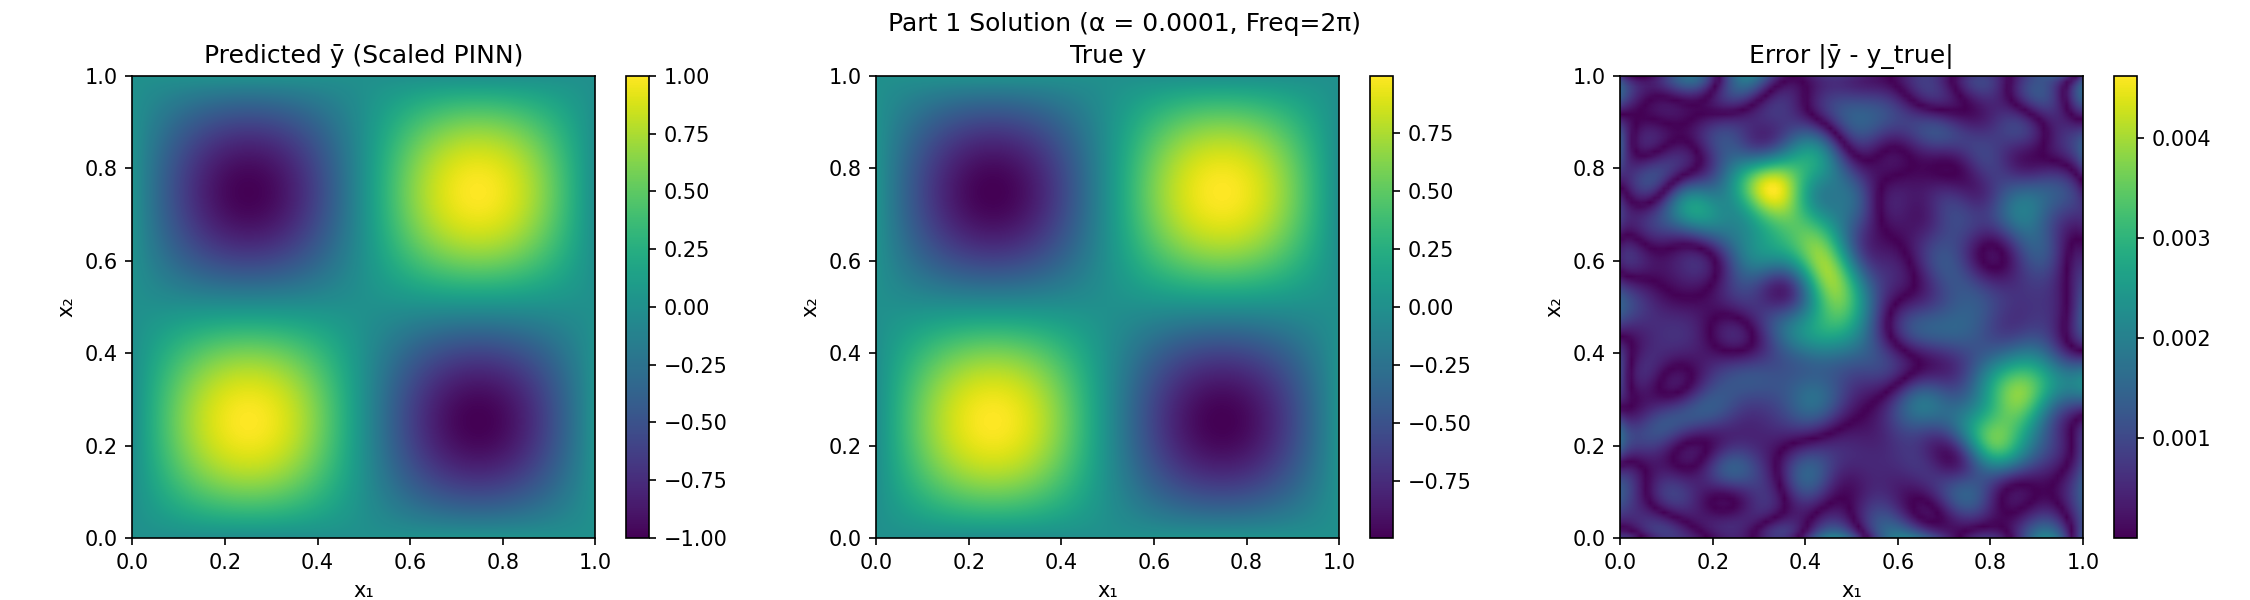
\includegraphics[width=\linewidth]{part1_solution_20260301_091035.png}
  \caption{Part 1 数值解与精确解对比}
  \label{fig:sol}
\end{figure}

\subsection{Fourier Feature Embedding 的引入}

在基本完成方法后，为排除过拟合，对 $f$ 进行了调整以测试模型的泛化能力。
在提高频率的过程中发现，模型对高频方程的处理能力不足，
于是加入了随机 Fourier 特征处理，使得模型在频率提高时依旧有良好表现。

\subsection{优化器 L-BFGS 的引入}

在加入 L-BFGS 之前，模型的误差量级虽然下降了，但结果一直处于震荡状态（图~\ref{fig:loss-no-lbfgs}）。

\begin{figure}[H]
  \centering
  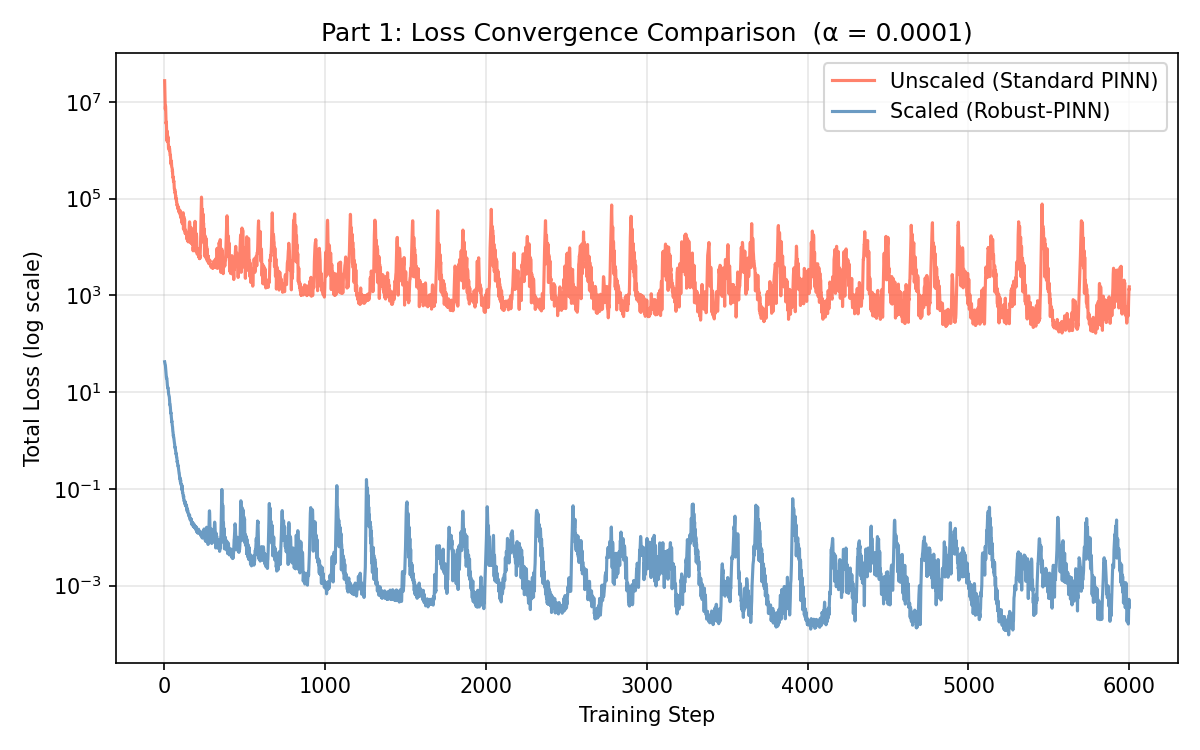
\includegraphics[width=0.8\linewidth]{part1_loss_comparison_20260301_085239.png}
  \caption{未使用 L-BFGS 时的损失曲线——收敛震荡明显}
  \label{fig:loss-no-lbfgs}
\end{figure}

在 PINN 经典论文~\cite{pinn_paper}及其参考文献~\cite{liu1989lbfgs}中，均选用了与 Adam
等一阶优化器不同的、更适合 PINN 损失函数的优化器——L-BFGS。其核心特性如下：

\begin{enumerate}[label=(\roman*)]
  \item \textbf{利用曲率信息（拟牛顿法）：}
    L-BFGS 通过保存历史梯度的变化，近似构造 Hessian 矩阵。
    当 $\mathrm{MSE}_u$ 和 $\mathrm{MSE}_f$ 的梯度相互拉扯导致普通优化器原地打转时，
    L-BFGS 能通过曲率信息"看穿"震荡，计算出使总损失同时下降的最优牛顿方向。

  \item \textbf{全批量评估（Full-batch）：}
    L-BFGS 是全批量算法——所有边界点和内部配点在每次迭代中完全固定并一次性输入。
    只有这样，损失函数的"地形"才是静止的，L-BFGS 的线搜索才能精准找到谷底。
\end{enumerate}

L-BFGS 的高收敛精度，使得物理残差正则化项被逼近机器精度，
从而在无网格划分（PINN 特性）的情况下，精准捕捉方程内部复杂的动态行为。


% ==================================================================


% ==================================================================


% ==================================================================
\begin{thebibliography}{9}

\bibitem{pinn_paper}
Raissi, M., Perdikaris, P., \& Karniadakis, G.\,E.\ (2019).
Physics-informed neural networks: A deep learning framework for solving forward and inverse problems involving nonlinear partial differential equations.
\textit{Journal of Computational Physics}, 378, 686--707.

\bibitem{liu1989lbfgs}
Liu, D.\,C.\ \& Nocedal, J.\ (1989).
On the limited memory BFGS method for large scale optimization.
\textit{Mathematical Programming}, 45(1-3), 503--528.

\end{thebibliography}

\end{document}